\SetPicSubDir{ch-Progressbar}
\SetExpSubDir{ch-Progressbar}

\chapter{Noticular: Near-peripheral and paracentral visualizations for OHMD notifications}
\chaptermark{Noticular}
\label{ch:Progressbar}




\section{Chapter overview}


This chapter explores the use of distinct visual regions to present OHMD notifications. To address the overarching research question (\autoref{sec:Intro:thesis_RQ}), \RQMainProgressBar{}, the underutilized paracentral and near-peripheral vision regions have been selected. To materialize the notification design, we examined progress notifications within a social setting, particularly face-to-face conversations (\autoref{sec:Progressbar:study_overview}). The primary question was then broken down into two main aspects for design and evaluation:
\begin{enumerate}
    \item How can progress notification content be distributed to the paracentral and near-peripheral vision during face-to-face conversations?
    \item How effective are such visualizations/designs in reducing the attention costs associated with progress notifications during face-to-face conversations?
\end{enumerate}


To address the first sub-question, we devised a circular progress bar, taking into account the anatomy of the human eye and insights derived from preliminary studies. Differing from traditional progress bar designs, we employed a circular layout to utilize the paracentral and near-peripheral vision and presented it intermittently rather than continuously.

To address the second sub-question, we evaluated this circular bar against commonly utilized textual and linear bars in a simulated conversational setting via a controlled experiment. We hypothesized that the circular bar would be less distracting due to its graphical nature and strategic placement surrounding the conversation partner than other types of progress bars. The results supported our hypothesis, indicating that the circular bar enabled users to maintain eye contact with their conversation partners while minimizing distractions from acquiring secondary information, thereby outperforming alternative solutions. We subsequently validated these findings in a realistic conversational setting, where the majority of participants continued to prefer the circular bar over other designs. We then explored potential applications of paracentral and near-peripheral visions for presenting secondary information on OHMDs. 

This chapter incorporates materials, including figures and tables, adapted from our pertinent research \cite{janaka_paracentral_2022}.











\section{Introduction}
\label{sec:Progressbar:introduction}

As discussed in \autoref{ch:Introduction} and \autoref{ch:Relatedwork}, it is crucial to minimize the adverse effects of notifications, particularly on OHMDs. OHMDs enable just-in-time information assistance anywhere and at any time \cite{hobert_application_2016, rhodes_just_time_2000, Klinker2018StructureFI}. For instance, OHMDs can augment social interactions by providing relevant information that closely aligns with users' immediate social contexts, such as conversation cues \cite{williams_designing_2015, nguyen_known_2015, tanveer_rhema_2015}. However, OHMD users may occasionally need to receive urgent secondary information, such as reminders about upcoming meetings or chat messages. This can negatively impact the quality of conversations and reduce eye contact \cite{mcatamney_examination_2006,  koelle_dont_2015}. 

This chapter outlines an approach aimed at mitigating such undesirable effects during social interactions. We emphasize minimizing the distraction caused by secondary information while maximizing users' attention on the primary viewing target (for example, the conversation partner) in social conversational settings. 
Building on the previous approach of distributing secondary information to different eye regions, we investigate two underexplored regions of our visual systems: the paracentral and near-peripheral vision (\autoref{sec:Relatedwork:central_peripheral_vision}). Additionally, we explore a secondary information visualization design that leverages their unique capabilities. We designed the circular progress bar, linear progress bar, and text labels and displayed them in the paracentral and near-peripheral regions of the eyes using an OHMD. These design alternatives were compared in a simulated and realistic conversational setting across two studies. The results suggest that the circular progress bar, designed to resemble the shape of our paracentral and near-peripheral vision, can more effectively utilize its capabilities. This allows users to perceive secondary progress updates with minimal distraction from their primary viewing task. Our studies also reveal intriguing insights that can inform the future design of attention-maintaining secondary visualizations for OHMDs, such as providing notification summaries and trip status updates.

The contributions of this chapter include: 1) a novel design for OHMD progress notifications that leverages paracentral and near-peripheral vision; 2) an evaluation of the proposed design against two common designs in both a simulated and realistic setting to understand the trade-offs between receiving notifications and maintaining the quality of social interactions. Based on these findings, we discuss potential OHMD designs to utilize paracentral and near-peripheral vision in other multitasking scenarios.












\section{Study overview}
\label{sec:Progressbar:study_overview}

To assess the potential of leveraging paracentral and near-peripheral vision for perceiving secondary information during social interactions (e.g., face-to-face conversations), we implemented three types of progress bars (\autoref{fig:Progressbar:study1:apparatus}, \autoref{fig:Progressbar:study2:apparatus}) to convey time information: a circular progress bar (\circularbar{}), a linear progress bar (\linearbar{}), and a text progress label (\textbar{}). We adopted recommendations from previous literature and conducted an informal pilot study with six participants in a conversational setting, testing various positions, colors, lengths, sizes, thicknesses, etc. The finalized design minimized distraction during conversations yet allowed comfortable acquisition of progress values.

The \textbar{} displays progress in a numerical format (0\% to 100\%), offering the most accurate presentation of progress quantity. Recognizing the importance of reading facial expressions and maintaining eye contact in social interactions \cite{hessels_how_2020, argyle1976gaze}, \textbar{} is positioned just above the conversation partner's head to avoid visual overlaps between the progress display and the partner's face. This location falls within the paracentral and near-peripheral vision (the precise position of gaze fixation determines which of the two vision types is utilized).

The \circularbar{} advances clockwise, beginning at 0\% and concluding at 100\% at the 12 o'clock position. It has a ring shape that fits within the natural viewing region of our eyes and suits the paracentral and near-peripheral vision. Considering the average head height\footnote{the vertical distance from the bottom of the chin to the top of the head} is approximately 26 cm for the 95th percentile \cite[Ch~B.8]{panero1979human}, the \circularbar{} has a 30 cm outer ring diameter and is 1 cm thick.

The \linearbar{} progresses from left (0\%) to right (100\%). It is straight, horizontally placed, and stretches across the two vision types. Like the \textbar{}, it is positioned just above the head with a thickness of 1 cm and a length of 40 cm.

As blue is visible in both the central and peripheral vision \cite{chaturvedi_peripheral_2019}, we used a blue color (\#FF0000FF in hex) to represent the completed progress, and a grey color (\#FF6B6B6B) for the incomplete portion in the \circularbar{} and \linearbar{}. The \textbar{} is displayed in sans-serif font following Debernardis et al. \cite{debernardis_text_2014} with a text height of 4 cm. All progress bars are displayed with the \textit{observer-locked} alignment as per Rzayav et al. \cite{rzayev_effects_2020}. The progress bars were positioned at the same focal distance (depth) as the conversational partner (i.e., digital character in \studyone{} and \observer{} in \studytwo{}) to prevent unnecessary focus switching.
  
There are trade-offs with using the three types of progress bars. Although \textbar{} provides an exact quantity that may permit higher accuracy, previous literature has shown that near-peripheral vision is less effective at recognizing text than shapes and symbols. The \circularbar{} and \linearbar{}, being graphical in nature, are thus easier to recognize via paracentral and near-peripheral vision. The areas on the screen occupied by these three progress types affect their noticeability and potential for distraction - as size increases, the noticeability improves, but it may become more distracting. The level of familiarity (e.g., users are more familiar with \linearbar{}) may also influence the perception of progress information.

We conducted two studies to formally investigate how these design trade-offs influence users' ability to perceive secondary information while focusing on the primary visual target. \Studyone{} (\autoref{sec:Progressbar:study1}) simulated a conversational setting with a digital character. This simulated setting was chosen to eliminate potential confounding factors inherent to real-world scenarios, allowing us to establish stronger causal relationships between stimuli and dependent measures. To verify the external validity of the results of \studyone{}, we also conducted \studytwo{} using a realistic conversation setting.















\section{Study 1:  Obtaining progress information while maintaining eye contact}
\label{sec:Progressbar:study1}

 
\Studyone{} explores how different progress \type{s} influence participants' ability to maintain eye contact and gather progress information. To circumvent eye-tracking inaccuracies arising from the head movement of the conversation partner, we used a simulated face-to-face conversation setting to measure eye contact, where participants focused on the facial features of a digital character.

\subsection{Participants}
\label{sec:Progressbar:study1:participants}

A total of 12 volunteers (7 females, mean age = 22.7 years, SD = 3.1) from the university community participated in the study. They had normal or corrected-to-normal visual acuity without any color deficiencies. Four participants had prior experience using OHMDs for less than 3 hours. Each participant was compensated approximately USD 7.25 per hour for their time.


\subsection{Apparatus}
\label{sec:Progressbar:study1:apparatus}

Participants wore the Microsoft HoloLens2\footnote{\url{https://www.microsoft.com/en-us/hololens/hardware}} (FoV = 52\textdegree{} diagonal, resolution = 1440x936 per eye, refresh rate = 60Hz, eye-tracking with 1.5-3\textdegree{} accuracy at 30Hz) as the OHMD platform. The HoloLens2 was chosen for its ability to display holograms at a specified distance and for not entirely obscuring the wearer's eyes. The progress display program was developed using Unity and MRTK\footnote{\url{https://github.com/Microsoft/MixedRealityToolkit-Unity}} for HoloLens2 and Python.

The digital character, a muted talking head video extracted and resized from the original video by docstocTV \cite{docstoctv_what_2014}, was displayed on a 27'' LCD monitor (refresh rate = 60 Hz, resolution = 1920 x 1080 px) at eye level (see \autoref{fig:Progressbar:study1:apparatus}). The progress bars were aligned relative to the digital character using fixed spatial coordinates.

The size of the face of the digital character was modeled after an average adult male (head height = 26 cm). To assist participants in maintaining eye contact with the video, we enabled a gaze cursor (a white dot) that dynamically tracked participants' gaze movements. We instructed participants to keep their gaze within a circular target region outlined in green (see \autoref{fig:Progressbar:study1:apparatus}). We ensured that the facial features of the digital character always remained within the target region for accurate eye-tracking.

The distance between the participant and the digital character was maintained at 1.5 m (\autoref{fig:Progressbar:study2:apparatus}), within the common range (1.2m - 3.6m) of natural social interactions as defined by Hall \cite{hall1966hidden, rzayev_effects_2020}. To prevent discomfort, we also adhered to the HoloLens design guidelines\footnote{\url{https://docs.microsoft.com/en-us/windows/mixed-reality/comfort}}.

The diameter of the target region (i.e., the green circle shown in \autoref{fig:Progressbar:study2:apparatus}) was set to 13 cm, covering the eyes and lips, ensuring that the visual angle, at a 1.5 m distance, falls within the central vision (eccentricity/visual angle of 2.5\textdegree{}). The \circularbar{} falls into the paracentral vision if a participant is focusing on the edges of the target region like the digital character's eyes (angle $\approx$ 3.2\textdegree{}), and falls into the near-peripheral vision if a participant is focusing on the center of the target region like the digital character's nose (angle $\approx$5.7\textdegree{}). The implementation details are at \autoref{sec:Progressbar:programming_codes}.

\begin{figure*}[hptb]
  \centering
  \includegraphics[width=1.03\linewidth]{\Pic{study1/study1_apparatus.pdf}}
  \caption[The apparatus in \studyone{}]{(a) The participants' view of the digital character and \circularbar{} through OHMD, (b) the \linearbar{} and \textbar{} as viewed by the participant, (c) visual angles when focused on the target focal region and the \circularbar{}. Depending on the focus location, the visual angles vary, making the progress bar visible from near-peripheral to paracentral vision, (d) the progress marking sheet given to participants. Original source of digital character by docstocTV \cite{docstoctv_what_2014}.}
  \label{fig:Progressbar:study1:apparatus}	  
\end{figure*}



\subsection{Task and procedure}
\label{sec:Progressbar:study2:task}

The study was conducted in a quiet room under indoor lighting conditions to ensure a consistent user experience. Upon entering the room, participants were briefed about the study procedure and signed a consent form. They were also acquainted with the OHMD and three types of progress bars, followed by an eye-tracking calibration. Throughout the experiment, they were instructed to maintain eye contact with the facial features of the digital character, even when progress notifications appeared.

The three progress type conditions were counterbalanced using a Latin Square design in a within-subject format. Each condition consisted of 15 trials. In each trial, a presentation type was assigned, and progress values (randomly chosen from 1-10, 20-30, ..., 90-100 bins with equal probability) were displayed on the OHMD while participants focused on the digital character. The character remained on screen for 7 seconds, with progress bars appearing for 1 second randomly between the 2$^{nd}$ and 5$^{th}$ seconds. These timings were based on participants' ability to identify shown progress while maintaining eye contact, as determined in a preliminary pilot study. Once the digital character disappeared, participants were asked to note down the progress value they had observed (see \autoref{fig:Progressbar:study1:apparatus}). They then proceeded to the next trial after a 3-second break.

Upon completing each condition, participants filled out a questionnaire about their experience during that condition. Two-minute breaks were provided between conditions to reduce fatigue. The entire experiment, including the post-questionnaire and interview, lasted approximately 50-60 minutes per participant.


\subsubsection*{Measures}
\label{sec:Progressbar:study1:measures}

In alignment with our RQs and \autoref{sec:Relatedwork:notification_evaluation}, we gauged the primary task performance as the quality of the simulated conversation and the secondary task (notification) performance as progress perception, using both objective and subjective measures.


\factor{Quality of the (simulated) conversation}  
For assessing the quality of conversation, we employed the Degree of Distraction (\distractionDigreee{} = $1 - $\textit{average percentage of times the user's gaze is within the target region}) as the objective measure. This metric evaluates the impact of notifications on maintaining eye contact, with a lower value indicating better performance. We also collected perceived task load data for maintaining eye contact and receiving progress information using Raw TLX (\perceivedTaskLoad{} measure assesses the perceived workload across six subjective subscales: Mental Demand, Physical Demand, Temporal Demand, Performance, Effort, and Frustration \cite{nasa_tlx_2006}), and \perceivedInterruption{} ('How much interruption did the progress bar cause to maintain eye contact when attempting to identify the progress?', 0-100 scale) as subjective measures.


\factor{Progress perception} 
For progress perception, we employed progress recognition accuracy (\progressAccuracy{} = $1 - avg(|progress_{displayed} - progress_{marked}|)$, progress values were shown in percentage) as the objective measure (the higher the value, the better). We also collected subjective measures such as \noticeability{} ('It was easy to notice the progress bar'), \perceivedEaseIdentification{} ('It was easy to identify the progress shown in the progress bar'), and \comfortability{} ('It was comfortable to check the progress while focusing on the face'), using 7-point Likert scales (1 = Strongly Disagree, 7 = Strongly Agree).

\factor{IRC framework}
All measures belong to the IRC framework \autoref{sec:Relatedwork:notification_evaluation}, as illustrated in \autoref{tab:Progressbar:study1:measures_IRC_mapping}. These are not explicitly mentioned above as they are grouped according to RQs.


\begin{table}[hptb]
\centering
\caption[Measures based on IRC framework]{Measures based on IRC framework. Here [O] represents objective measures while [S] represents subjective measures.}
\label{tab:Progressbar:study1:measures_IRC_mapping}
\small
\begin{tabular}{@{}ll@{}}
\toprule
Parameter & Measures \\ \midrule
\Interruption{} &  [O] \distractionDigreee{} \\
     &  [S] \perceivedTaskLoad{}, \perceivedInterruption{} \\
\Reaction{} &  [S]  \noticeability{} \\
\Comprehension{} &  [O] \progressAccuracy{} \\
    & [S] \perceivedEaseIdentification{} \\
% \cmidrule(lr){2-2}
\Satisfaction{}  & [S] \preference{}, \comfortability{}  \\ 
\bottomrule
\end{tabular}
\end{table}

\subsection{Results}

During the study, each participant completed three testing conditions, resulting in a total of 45 trials per participant. This yielded a total of 540 ( = 12 x 3 x 15) data points. The mean performance related to the quality of conversation is depicted in \autoref{fig:Progressbar:study1:box_results_distraction} and summarized in \autoref{tab:Progressbar:study1:mean_results_distraction}. Similarly, the participants' mean performance concerning progress perception is presented in \autoref{fig:Progressbar:study1:box_results_recognition} and summarized in \autoref{tab:Progressbar:study1:mean_results_recognition}.

\subsubsection*{Analysis}
\label{study1:analysis}

We conducted a one-way repeated measures ANOVA or Friedman test (if ANOVA assumptions were violated) on the quantitative data. Normality and sphericity were tested using the Shapiro-Wilk test and Mauchly's test, respectively. For post-hoc tests, we used multiple means comparisons with Bonferroni correction for the parametric data and pairwise Wilcoxon signed-rank tests with Bonferroni correction\footnote{Note: Bonferroni-corrected \pval{} values are indicated as \pbonf{}. \pbonf{} is calculated by multiplying the observed (uncorrected) \pval{} by the number of comparisons made \cite{Bland170, ibm_calculation_2023}.} for non-parametric data. When non-parametric distributions could take a broad range of values (e.g., RTLX, which ranged from 0-100) and satisfied parametric assumptions, we employed parametric tests. The interview recordings were transcribed and analyzed thematically following Braun and Clarke \cite{braun_using_2006}.


\subsubsection*{Task feedback} 

During the study, all participants tended to focus on the eyes, nose, nostrils, or mouth of the digital character based on their habitual conversation behaviors. All participants reported that focusing on the target region positioned at the center of the digital character's face and noting the progress was \quote{quite easy}. They also found the progress bars visibly prominent when directly observed. The majority felt that the duration indicated by the progress bar was adequate. However, four participants expressed a preference for more time with the \textbar{}, stating that even with additional time, they might struggle to recognize the text while focusing on the face. During the post-study interview, all participants agreed that the gaze cursor aided in maintaining focus on the target region without hindering their recognition of the progress values.


\begin{figure*}[hptb]
\centering

\begin{subfigure}{0.47\textwidth}
  \centering
  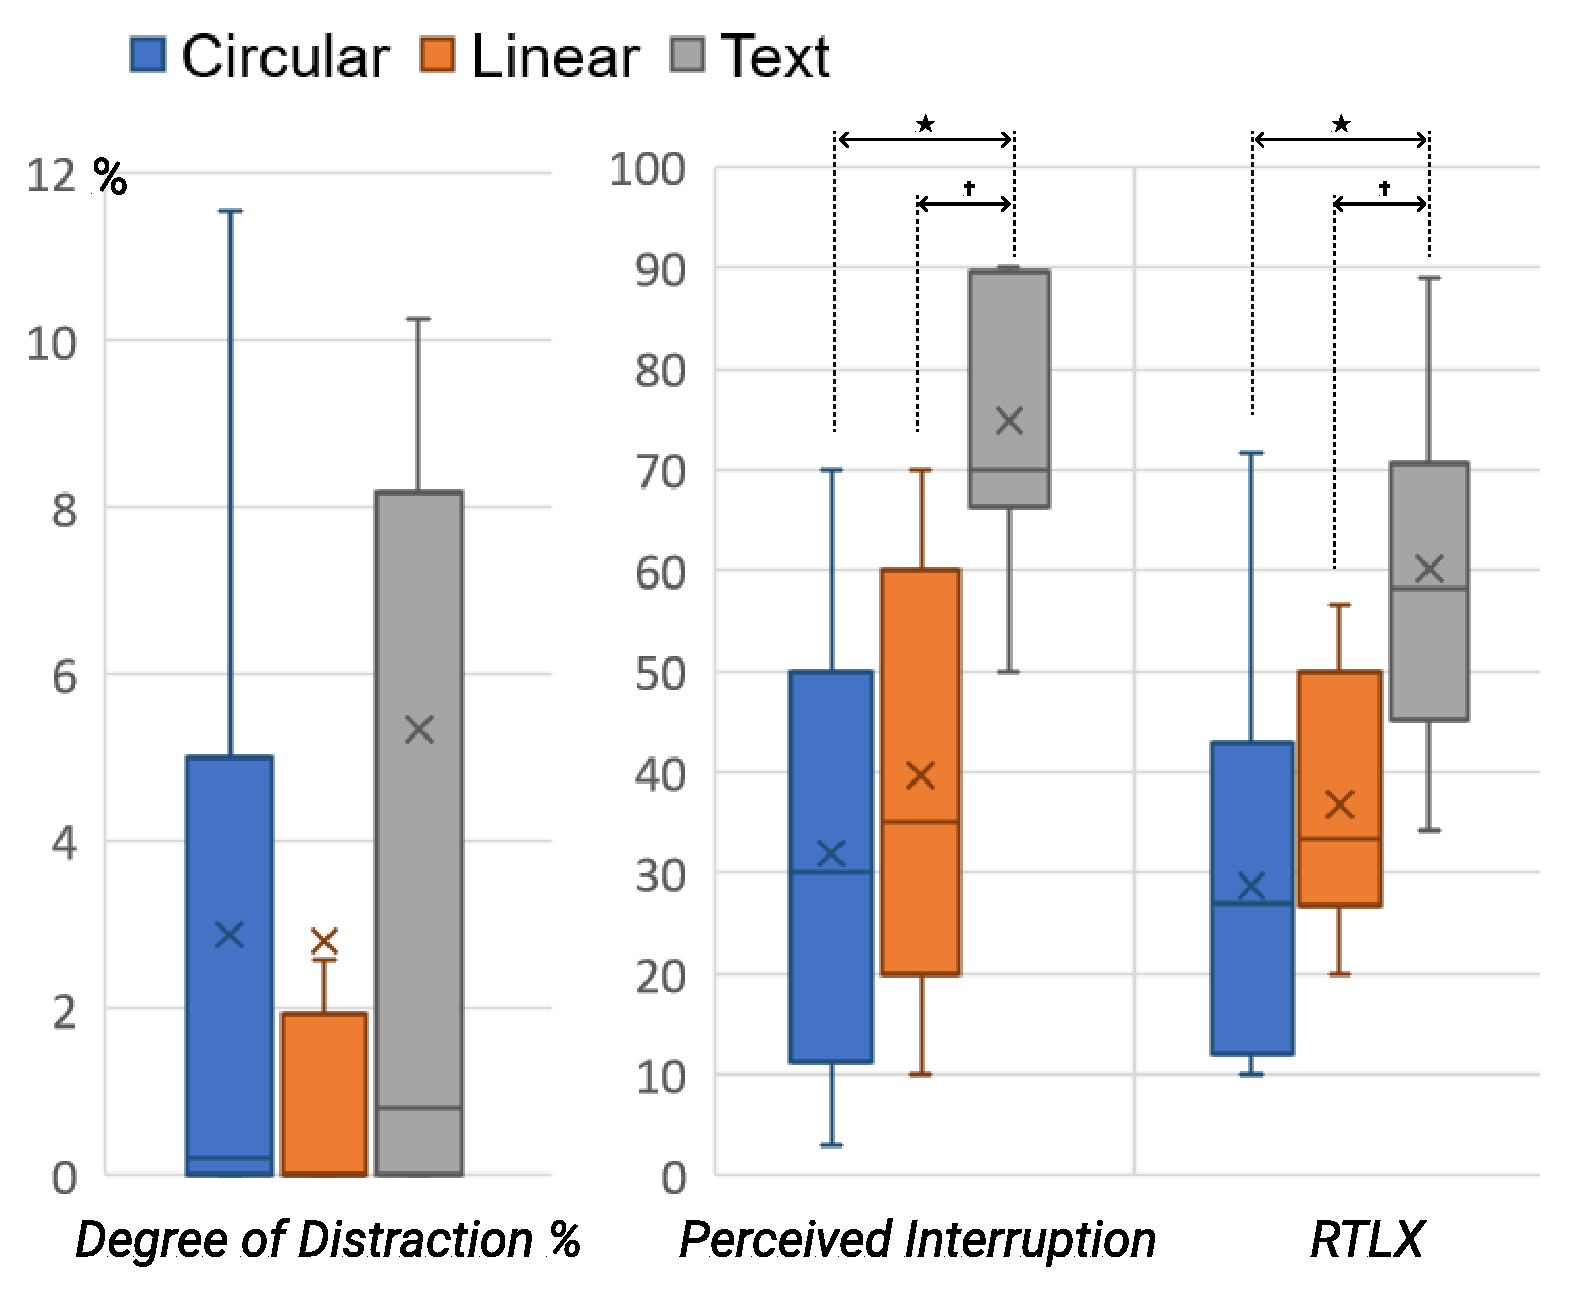
\includegraphics[width=\linewidth]{\Pic{study1/study1_box_quality_conversation.pdf}}
  \caption{Quality of conversation}
  \label{fig:Progressbar:study1:box_results_distraction}
\end{subfigure}%
\begin{subfigure}{0.57\textwidth}
  \centering
  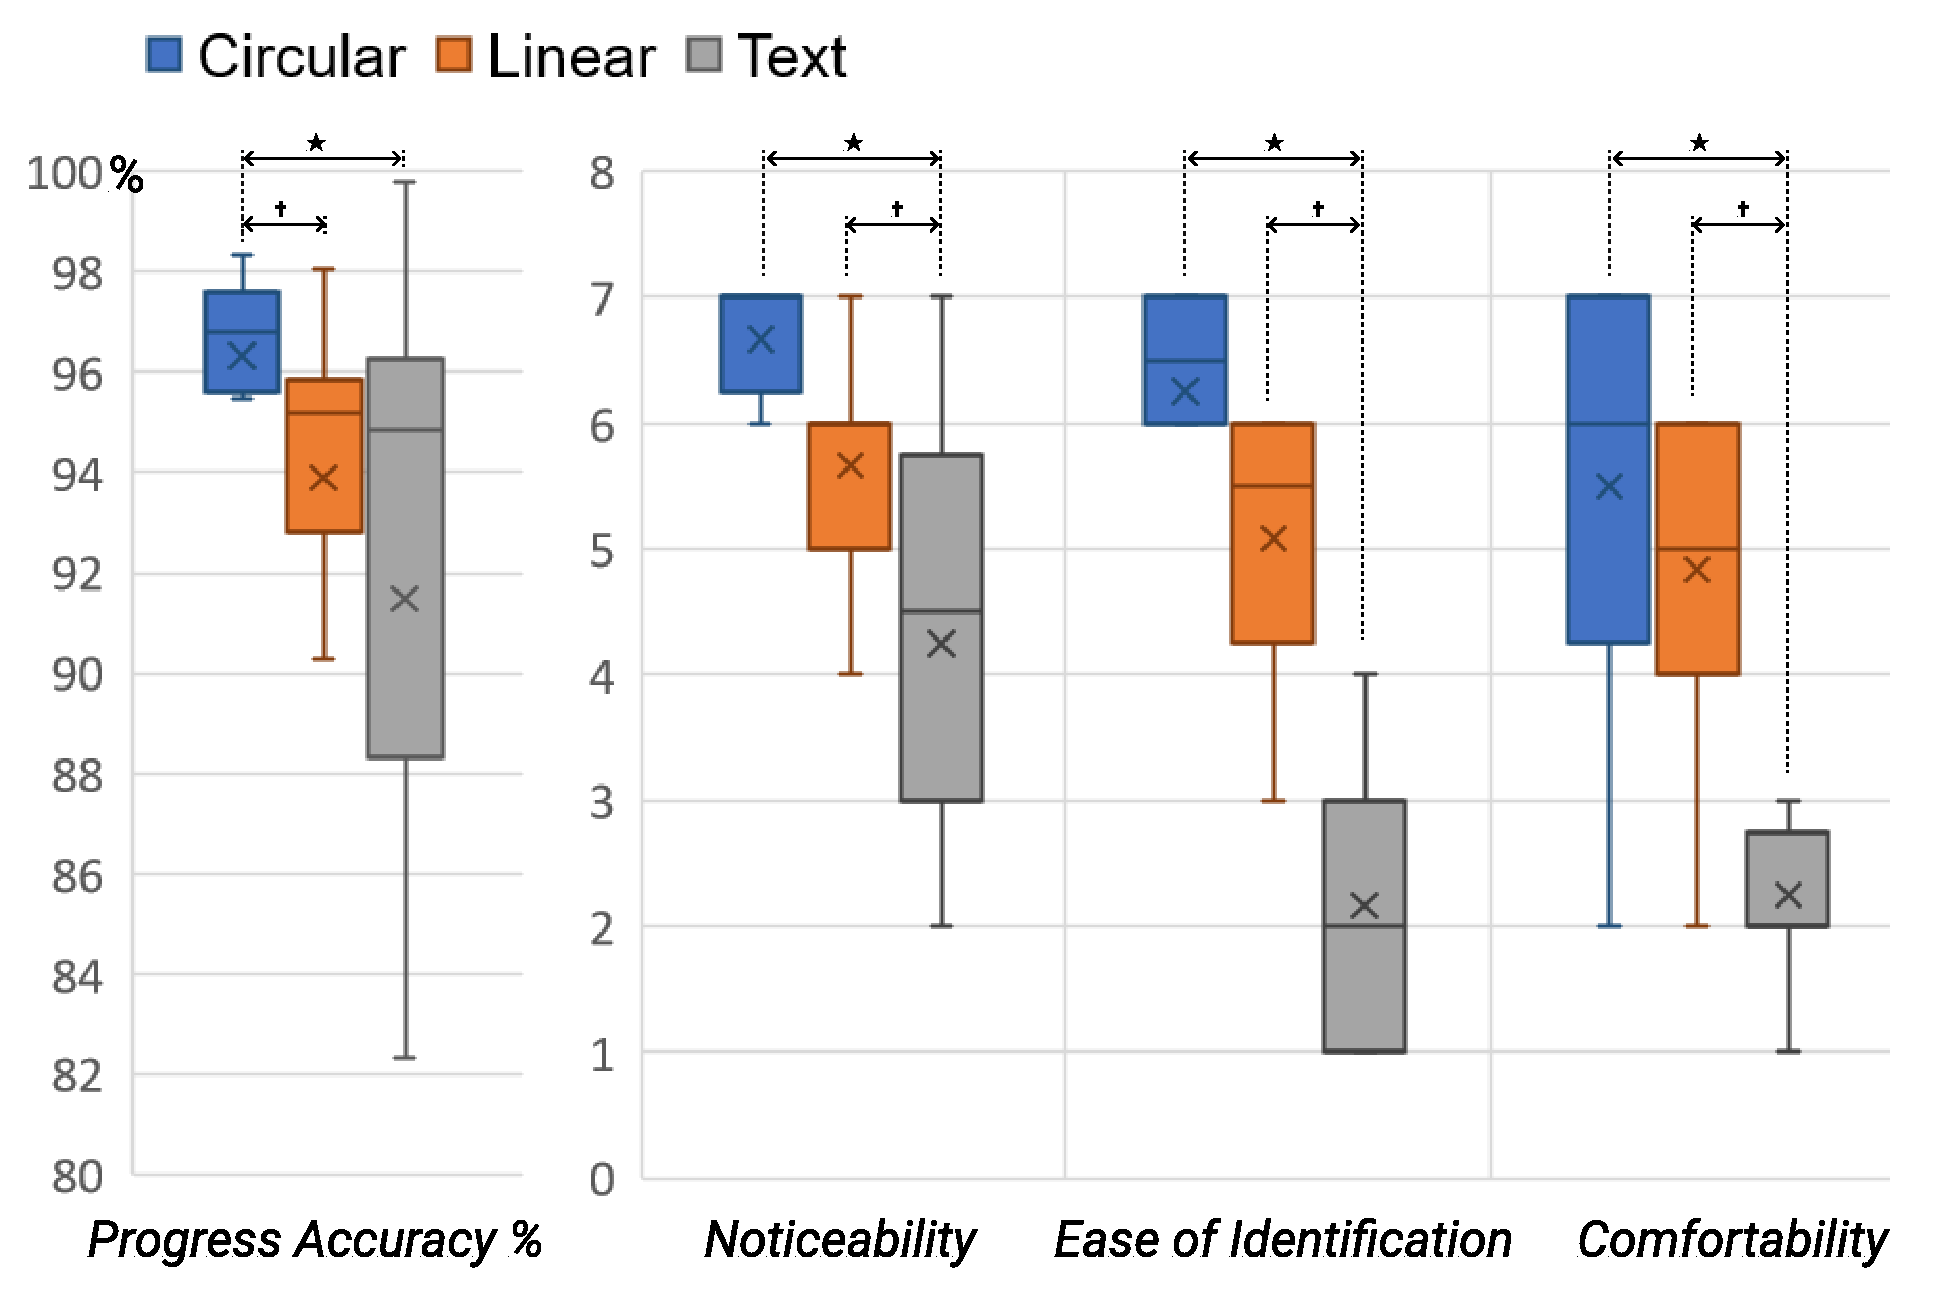
\includegraphics[width=\linewidth]{\Pic{study1/study1_box_progress_perception.pdf}}
  \caption{Progress perception}
  \label{fig:Progressbar:study1:box_results_recognition}
\end{subfigure}

\caption[Average performance in \studyone{}]{Measures in the simulated conversation setting (N = 12). \significantI{} and \significantII{} represent significant (\pval{<0.05}) post-hoc tests and  $\times$ inside box plot represents the mean value point. See \autoref{tab:Progressbar:study1:mean_results_recognition} and \autoref{tab:Progressbar:study1:mean_results_distraction} for details. }
\label{fig:Progressbar:study1:box_results}
\end{figure*}




\subsubsection*{Quality of conversation (primary task performance).}

\autoref{fig:Progressbar:study1:box_results_distraction} (\autoref{tab:Progressbar:study1:mean_results_distraction}) provides a summary of the measures.

\begin{table*}[hptb]
\centering
\caption[Primary task performance in \studyone{}]{Quality of conversation in simulated conversation setting (N = 12). Colored bars show the relative value of each measure for different progress \type{s}. \significantI{} and \significantII{} represent significant (\pval{<0.05}) post-hoc tests.}
\label{tab:Progressbar:study1:mean_results_distraction}
\small
\begin{tabular}{@{}l|ll|ll|ll@{}}
\toprule
\multicolumn{1}{r}{Measure} &
  \multicolumn{2}{c}{\distractionDigreee{} \%} &
  \multicolumn{2}{c}{\perceivedInterruption{}} & 
  \multicolumn{2}{c}{\perceivedTaskLoad{}} \\ \cmidrule(l){2-7} 
\multicolumn{1}{l}{Format} &
  \multicolumn{1}{l}{M} &
  \multicolumn{1}{l}{SD} &
  \multicolumn{1}{l}{M} &
  \multicolumn{1}{l}{SD} &
  \multicolumn{1}{l}{M} &
  \multicolumn{1}{l}{SD} \\ \midrule
  
\Circularbar{} & 
\databar{7}{2.88} & 4.74 &
\databar{80}{31.92}\significantI{} & 23.42 & 
\databar{70}{28.75}\significantI{} & 18.82 \\

\Linearbar{} & 
\databar{7}{2.81} & 7.47 & 
\databar{80}{39.75}\significantII{} & 22.32 & 
\databar{70}{36.81}\significantII{} & 12.58  \\

\Textbar{} & 
\databar{7}{5.35} & 10.75 & 
\databar{80}{74.92}\significantI{}\significantII{} & 13.55 &   
\databar{70}{60.21}\significantI{}\significantII{} & 16.54  \\
\bottomrule
\end{tabular}
\end{table*}

\factor{Objective measure - \distractionDigreee{}} 

Despite there being no significant difference (\friedman{2}{3.257}{=0.196}{0.703}) among progress \type{s}, \textbar{} registered the highest average value for \distractionDigreee{}.

\factor{Subjective measures - \perceivedInterruption{} and \perceivedTaskLoad{}}

Overall, \circularbar{} recorded lower \perceivedInterruption{} and \perceivedTaskLoad{}. Repeated-measures ANOVAs revealed significant effects of \perceivedInterruption{} (\anovawef{2}{22}{21.026}{<0.001}{0.657}) and \perceivedTaskLoad{} (\anovawef{2}{22}{16.646}{<0.001}{0.602}). Post-hoc analyses disclosed that \textbar{} was significantly different (higher, \pbonf{<0.01}) from \linearbar{} and \circularbar{} in terms of \perceivedInterruption{} and \perceivedTaskLoad{}. Results for individual indices of \perceivedTaskLoad{} are presented in \autoref{fig:Progressbar:study1:nasa_tlx}. A post-hoc analysis with Bonferroni correction showed that for all measures, \circularbar{} and \linearbar{} yielded significantly lower (\pval{<0.05}) task load results than \textbar{}. However, there were no significant differences between \circularbar{} and \linearbar{}, even though \circularbar{} recorded the lowest average task loads for all measures. On all indices, including the overall score, the sorted order of task load from lower to higher was: \circularbar{} < \linearbar{} < \textbar{}.

\begin{figure}[hptb]
  \centering
  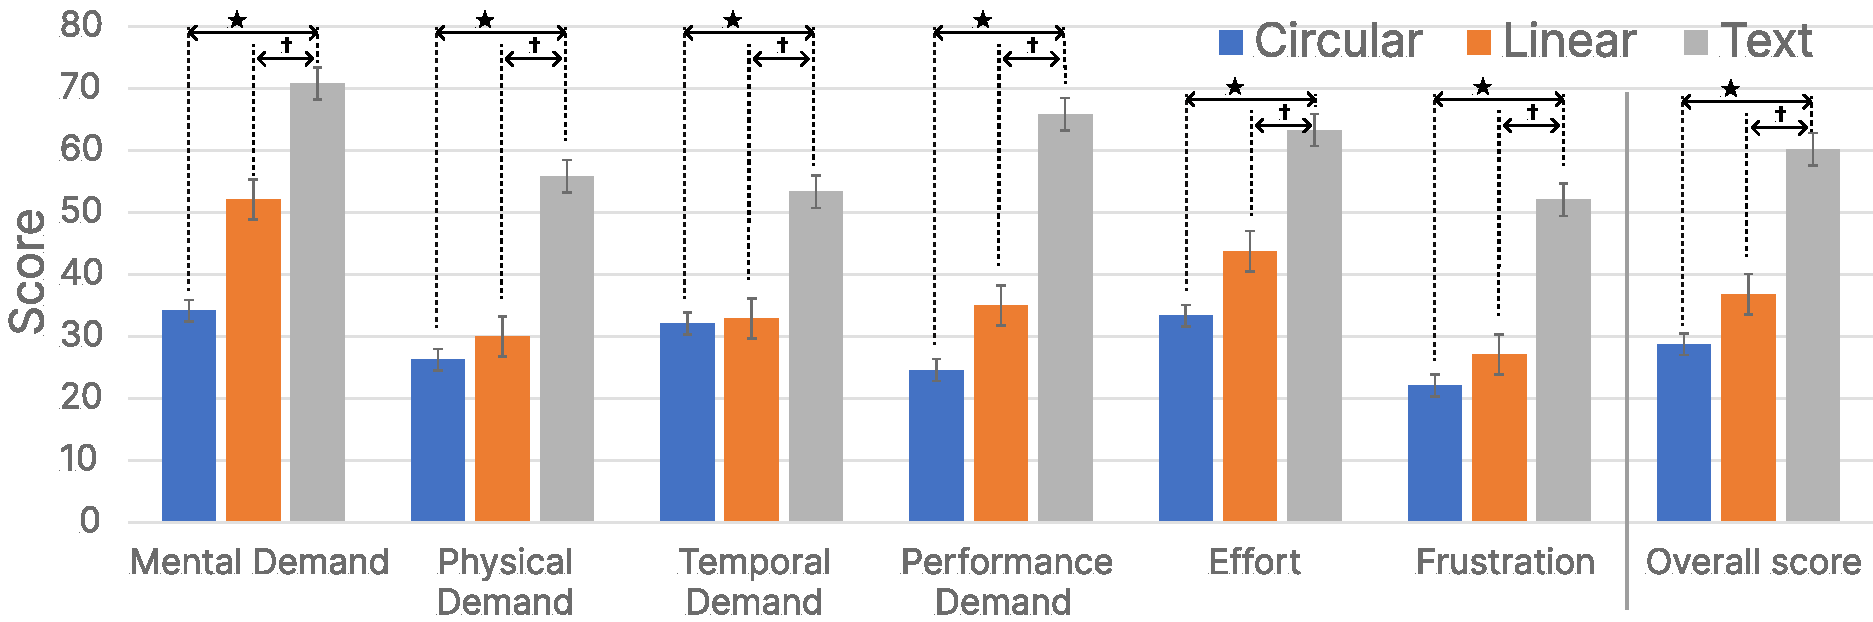
\includegraphics[width=0.9\linewidth]{\Pic{study1/study1_nasa_tlx.pdf}}
  \caption[NASA-TLX scores in \studyone{}]{NASA-TLX scores for \circularbar{}, \linearbar{}, and \textbar{}. Overall \circularbar{} had the lowest \perceivedInterruption{}. \significantI{} and \significantII{} represent significant (\pbonf{<0.05}) post-hoc tests. Error bars represent standard errors.}
  \label{fig:Progressbar:study1:nasa_tlx}	  
\end{figure}

Furthermore, all participants ranked \textbar{} as the most distracting \type{}, citing difficulty in reading or \quote{figuring out} numbers in the periphery and that it often led them to shift their focus away from the face. The majority of participants (10/12) selected \circularbar{} as the least distracting since it allowed them to perceive progress notifications without disruptions in focus.



\subsubsection*{Progress perception (notification task performance).}


\autoref{fig:Progressbar:study1:box_results_recognition} (\autoref{tab:Progressbar:study1:mean_results_recognition}) provides a summary of the measures.


\begin{table*}[hptb]
\centering
\caption[Secondary task performance in \studyone{}]{Progress perception measures in the simulated conversation setting (N = 12). Colored bars show the relative value of each measure for different progress \type{s}. \significantI{} and \significantII{} represent significant (\pbonf{<0.05}) post-hoc tests.}
\label{tab:Progressbar:study1:mean_results_recognition}
\small
\begin{tabular}{@{}l|ll|ll|ll|ll@{}}
\toprule
\multicolumn{1}{r}{Measure} &
  \multicolumn{2}{c}{\progressAccuracy{} \%} &
  \multicolumn{2}{c}{\noticeability{}} &
  \multicolumn{2}{c}{\perceivedEaseIdentification{}} &
  \multicolumn{2}{c}{\comfortability{}} \\ \cmidrule(l){2-9} 
\multicolumn{1}{l}{Format} &
  \multicolumn{1}{l}{M} &
  \multicolumn{1}{l}{SD} &
  \multicolumn{1}{l}{M} &
  \multicolumn{1}{l}{SD} &
  \multicolumn{1}{l}{M} &
  \multicolumn{1}{l}{SD} &
  \multicolumn{1}{l}{M} &
  \multicolumn{1}{l}{SD} \\ \midrule
  
\Circularbar{} & 
\databarrel{100}{80}{96.32}\significantI{}\significantII{} & 2.15 & 
\databar{7}{6.67}\significantI{}\significantII{} & 0.65 &
\databar{7}{6.25}\significantI{} & 1.14 & 
\databar{7}{5.50}\significantI{} & 1.68 \\

\Linearbar{} & 
\databarrel{100}{80}{93.89}\significantI{} & 3.82 & 
\databar{7}{5.67}\significantII{} & 0.99 & 
\databar{7}{5.08}\significantII{} & 1.17 & 
\databar{7}{4.83}\significantII{} & 1.19 \\

\Textbar{} & 
\databarrel{100}{80}{91.47}\significantII{} & 8.71 & 
\databar{7}{4.25}\significantI{} & 1.66 & 
\databar{7}{2.17}\significantI{}\significantII{} & 1.12 & 
\databar{7}{2.25}\significantI{}\significantII{} & 0.75 \\
\bottomrule
\end{tabular}
\end{table*}


\factor{Objective measure - \progressAccuracy{}} 

Overall, when participants maintained eye contact, the accuracy of progress identification dropped significantly for \textbar{} (\range{68.2}{99.8}) compared to \circularbar{} (\range{90.2}{98.3}) or \linearbar{} (\range{83.5}{98.1}). The Friedman test disclosed a significant effect (\friedman{2}{10.167}{=0.006}{0.618}) of \type{}. Surprisingly, post-hoc analysis indicated that \circularbar{} was significantly higher (\pbonf{<0.05}) than \linearbar{} and \textbar{} in terms of \progressAccuracy{}.
 
Notably, \textbar{} registered the highest variation in average accuracy, as participants' estimation errors were either very high or very low. All participants found it \quote{very difficult} to recognize and distinguish digits, as they appeared \quote{blurry} or \quote{hazy} when not looking at them directly. Specifically, they found \quote{curved} numbers (e.g., 3, 6, 8, 9) harder to recognize than \quote{pointy} ones (e.g., 1, 4). Nonetheless, two participants could achieve almost full accuracy for \textbar{} while focusing on the face, indicating individual differences in the ability to read text in the paracentral vision. Similarly, a few participants found the extreme ends of \linearbar{} (further away from the central vision) harder to read. Conversely, most participants perceived that the \circularbar{} was easier to correctly recognize the position of, as it was larger and had an additional element of \quote{angle}, e.g., 25\% is at a 90\textdegree{} angle from the center, which made the progress position more obvious.


\factor{Subjective measures - \noticeability{}, \perceivedEaseIdentification{}, and \comfortability{}}

\Circularbar{} recorded the highest average ratings for \noticeability{}, \perceivedEaseIdentification{}, and \comfortability{}. Friedman tests revealed significant effects of \noticeability{} (\friedman{2}{14.6}{<0.001}{0.388}),  \perceivedEaseIdentification{} (\friedman{2}{21.56}{<0.001}{0.307}), and \comfortability{} (\friedman{2}{16.13}{<0.001}{0.578}). Post-hoc analyses showed that \circularbar{} was significantly different (higher, \pbonf{<0.05}) from both \linearbar{} and \textbar{} in terms of \noticeability{}. Similarly, \textbar{} was significantly different (lower, \pbonf{<0.05}) than \linearbar{} and \circularbar{} in terms of \perceivedEaseIdentification{} and \comfortability{}.

The majority (10/12) of participants indicated that the \circularbar{}, which appears around the face with a larger area, was more noticeable than the \textbar{} or \linearbar{}, making it easier for them to identify the progress.



\subsubsection*{Preference}

The majority of participants (10/12) ranked \circularbar{} as their most preferred progress type, with \textbar{} being the least preferred. In our interview, participants reported that the surrounding shape of the \circularbar{} allowed them to identify the displayed progress without moving their gaze\footnote{This was further confirmed by visualizing the gaze trajectory as well.}, making it more comfortable to look at while maintaining eye contact. Additionally, the \circularbar{} resembled the familiar \quote{clock} with the progress shown at an \quote{angle}. Given its larger size, they were able to perceive the progress notifications with greater accuracy.

The remaining participants (2/12) who chose the \linearbar{} as their preferred option reported that the fixed location of the \linearbar{} allowed them to track progress values more easily than the \circularbar{} since progress values could appear anywhere around the face.

All participants chose the \textbar{} as the least preferred option, stating that the \textbar{} was \quote{difficult to decipher} (i.e., distinguish digits) and required them to exert more effort to interpret the numbers (in paracentral and near-peripheral vision) while keeping their gaze on the face.

\subsection{Discussion}

Surprisingly, evidence suggests that \textbar{} does not provide higher accuracy, as \circularbar{} demonstrated significantly higher \progressAccuracy{} and \perceivedEaseIdentification{} than \textbar{}. Text can only be clearly perceived when presented within central vision \cite{rayner_eye_1998, ishiguro_peripheral_2011}, which was not the case for our \textbar{} condition.

Given that both \circularbar{} and \linearbar{} have simpler visual patterns than text \cite[Ch~6]{wickens_engineering_2015}, and that shapes and colors are recognized at a greater angle than text \cite[Ch~C.9]{ishiguro_peripheral_2011, panero1979human}, the \circularbar{} and \linearbar{} were easier to recognize in paracentral and near-peripheral vision than the \textbar{}.

As expected, the \circularbar{} had significantly lower \perceivedInterruption{}, \perceivedTaskLoad{}, and a lower \distractionDigreee{} than \textbar{}. We lack evidence to draw the same conclusion for the comparison between \circularbar{} and \linearbar{}.

Comparing \textbar{} with \circularbar{}, there appears to be a trade-off between accuracy and maintaining (uninterrupted) eye contact for \textbar{}. A majority (83\%) of participants preferred the \circularbar{}, in line with the results showing that \circularbar{} resulted in the lowest distraction levels and highest accuracy while participants maintained uninterrupted eye contact. Hence, the \circularbar{} is the ideal choice for presenting progress/task completion reminders when users need to maintain their focus on a primary visual target.























\section{Study 2: Identify how the presentation type of progress notifications affect face-to-face conversations}
\label{sec:Progressbar:study2}

In this study, we complemented \studyone{} with a more realistic setting in which a pair of participants (\receiver{} and \observer{}, \autoref{sec:Progressbar:study2:apparatus}) engaged in a conversation. We initially explored the optimal form of \persistence{} (i.e., whether progress is presented \continuous{ly} or \intermittent{ly} on the OHMD) for progress bar design through a pilot study with 4 participants, then subsequently conducted a formal study with 12 participants.


\subsection{Apparatus}
\label{sec:Progressbar:study2:apparatus}

As shown in \autoref{fig:Progressbar:study2:apparatus}, the same HoloLens2 was used by the \receiver{}, where the progress information was displayed in an observer-locked alignment with the face of the \observer{}. This observer-locked alignment was implemented using Windows' FaceTracker\footnote{\url{https://docs.microsoft.com/en-us/uwp/api/Windows.Media.FaceAnalysis.FaceTracker}} API and Unity's viewport to world mapping\footnote{\url{https://docs.unity3d.com/ScriptReference/Camera.ViewportToWorldPoint.html}} at a fixed distance with a tracking rate of 10Hz. To minimize misalignments of progress bars with respect to the \observer{} due to tracking errors, we asked trained \observer{s} to limit their \textit{sudden} head movements during conversations. The gaze cursor was removed for realistic effects, as they are rarely used in real conversations. The distance between the \receiver{} and \observer{} was maintained at 1.5 m, replicating \studyone{}. 


\begin{figure}[hptb]
  \centering
  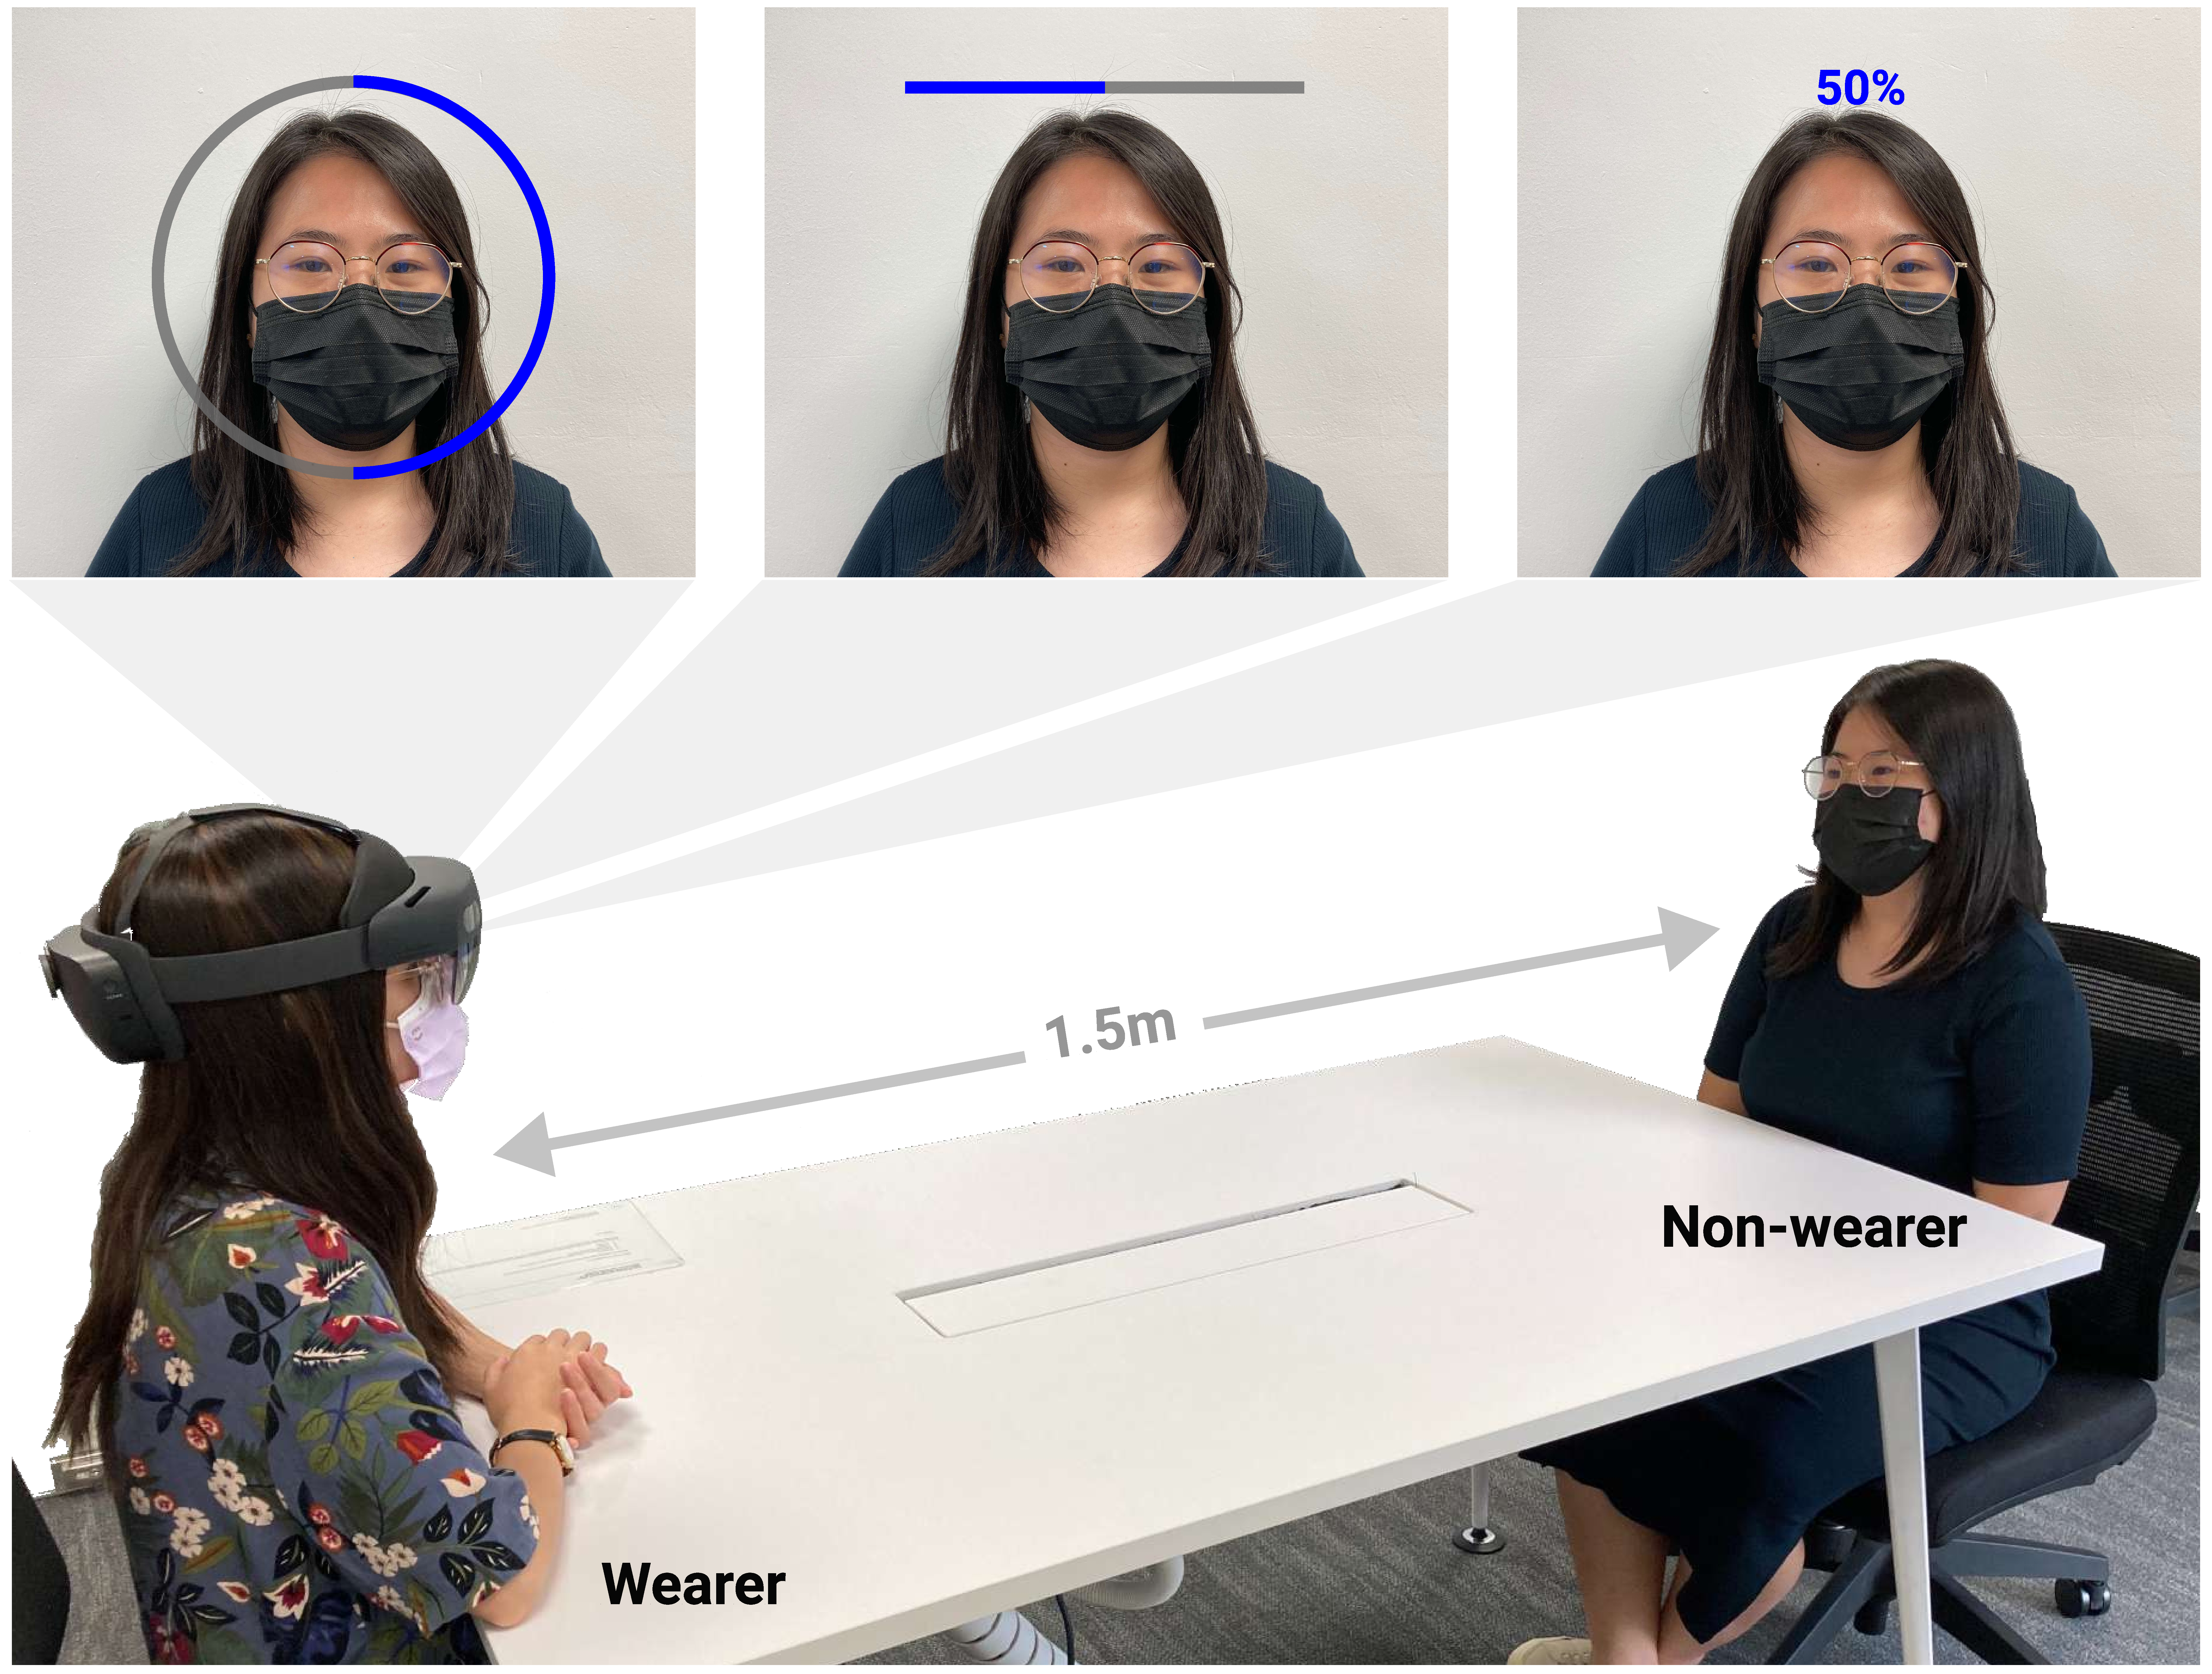
\includegraphics[width=0.8\linewidth]{\Pic{study2/study2_apparatus.pdf}}
  \caption[The apparatus in \studytwo{}]{The \receiver{} is wearing the OHMD while engaging in a conversation with the \observer{}. The \receiver{} sees three progress \type{s} in three conditions. From left to right, the top figure depicts the progress bars: \circularbar{}, \linearbar{}, and \textbar{}.}
  \label{fig:Progressbar:study2:apparatus}
\end{figure}


\subsection{Tasks}
 
A \receiver{} and \observer{} pair engaged in a face-to-face conversation on a given topic (\autoref{fig:Progressbar:study2:apparatus}) provided by the researcher. The topics were selected from the CAE speaking test \cite{cambridge2008speaking} (e.g., ``What are the advantages and disadvantages of shopping by computer?''), similar to those used by Mayer et al. \cite{mayer_evaluating_2018} and Rzayev et al. \cite{rzayev_effects_2020}. We limited each conversation session to 6 minutes, ensuring that participants had sufficient time to engage in the conversation and attend to progress notifications. 

In addition to engaging in the conversation as the primary task, both the \receiver{} and the \observer{} had secondary tasks. We asked the \receiver{} to end the conversation smoothly when the progress bar reached 100\% and then stand up. The \observer{} was instructed to observe whether the \receiver{} paid attention to the conversation and to rate the eye contact and naturalness of the conversation after the discussion. Neither was aware of the other's secondary task.

\subsection{Progress bar design}

\subsubsection*{General design}

In order to establish the conversation flow, we started the progress bar from 0\% 30 seconds after the conversation began. The progress bars then incremented at a uniform speed of 1\% every 3 seconds, reaching 100\% in 5 minutes. After this, the progress bar remained on view for an additional 45 seconds before it informed the \receiver{} to stop the session.

\subsubsection*{Pilot study to determine the persistence}
\label{study2:pilot_persistance}

We tested two kinds of \persistence{} for progress notification presentation: \continuous{} and \intermittent{}. The \continuous{} progress bar remained on the screen, whereas the \intermittent{} progress bar appeared only when the progress value reached multiples of 10\% (i.e., 10\%, 20\% ...), staying on the screen for 3 seconds each time it appeared. The appearance interval and staying duration were determined by several pilots.

The pilot results with 4 participants showed that the \continuous{} \persistence{} on screen was perceived as more distracting and was less preferred compared to the \intermittent{} one. Participants reported that they tended to \quote{constantly check the progress}, as the value was continuously changing, and they did not intend to do this, especially when they had more time left for conversation. This constant checking disrupted their \quote{train of thoughts}. As for preference, most participants (3/4) preferred \intermittent{}, as it highlighted progress with minimal distraction. This finding aligns with the literature \cite{tanveer_rhema_2015, ofek_reducing_2013} that recommends sparse feedback to reduce distraction from the primary task during multitasking. The only participant who reported more distraction from the \continuous{} still preferred it due to the accurate time tracking. Based on the pilot results, we decided to use only the \intermittent{} \persistence{} in the formal study.

\subsection{Participants}
\label{sec:Progressbar:study2:participants}
 
The \receiver{s} were 12 participants (7 females, mean age = 22.4, SD = 2.5) recruited from the university community, following the same standards as \studyone{} (\autoref{sec:Progressbar:study1:participants}). The \observer{s} were two volunteers (2 males, mean age = 24.5) from the same community and were trained to manage the conversation to ensure fluid continuity. They were fluent in English and acted as conversation partners. The \observer{s} were not aware of the study conditions. None of them participated in \studyone{}. 


\subsection{Procedure}
 
The study was conducted in a quiet room under indoor lighting conditions to provide a consistent user experience. When the \receiver{s} arrived, they were briefed about the study process and signed the consent form. They then familiarized themselves with the OHMD and the three types of progress bars. They were also informed about the intermittent appearance, expected duration, and frequency of the progress bar during the conversation. They were reminded to focus on the conversation while attending to the progress bars. 

When the \receiver{} was comfortable with the setup, the \observer{} was guided to the same room and seated on the opposite side of a table (see \autoref{fig:Progressbar:study2:apparatus}) such that they were 1.5 m apart from each other. They were given a practice topic to engage in a conversation without any progress bar displayed on the OHMD for 3-4 minutes. They then engaged in three conversation sessions with three types of progress bars. After each conversation, the \receiver{} removed the OHMD, and the participant pair filled out the questionnaires (\autoref{sec:Progressbar:study2:measures}) separately. After completing the questionnaire, a 2-minute break was provided before proceeding to the next condition. In the end, both participants filled out a questionnaire on their overall experience and separately attended the semi-structured interview sessions. These sessions captured the \receiver{'s} perception of progress indication, their experience of receiving progress notifications, and the \observer{'s} perception of the conversation. The study took approximately 80 minutes per participant pair.

\subsection{Study design}

We tested three conditions: the \circularbar{}, \linearbar{}, and \textbar{} using a within-subject design, which was fully counterbalanced.



\subsubsection*{Measures}
\label{sec:Progressbar:study2:measures}

In this study, we collected subjective measures of the quality of two-way conversation and the \receiver{'s} perception towards the different progress \type{s}. At the end of the study, we also collected the \receiver{s'} preference for different progress types.

\factor{Quality of the conversation}
To measure the quality of the conversation, we employed three categories of measures: attention and concentration, eye contact, and naturalness; these were gathered from both the \receiver{'s} (\prefixReceiver{}) and \observer{'s} (\prefixObserver{}) perspectives. These measures were adapted from McAtamney et al.'s study \cite{mcatamney_examination_2006}, but the 5-point Likert scales were changed to 7-point scales (1 = Strongly Disagree, 7 = Strongly Agree) to increase sensitivity and ensure consistency with other measures (see \autoref{tab:Progressbar:study2:scales_conversation} for the list of measures used in the study).


\begin{table*}[hptb]
\centering
\caption[Additional measures on conversation quality]{Aspects and measures on conversation behavior of \receiver{} from the \receiver{} \prefixReceiver{} and the \observer{} \prefixObserver{} point of views (source: \cite{mcatamney_examination_2006}).}
\label{tab:Progressbar:study2:scales_conversation}
\small
\begin{tabular}{l p{0.7\textwidth} }
\toprule
Aspect on conversation                     & Measures                  \\ \midrule
\multirow{2}{*}{\begin{tabular}[c]{@{}l@{}} Attention and \\concentration\end{tabular}} 

& \b{AC1}: {\prefixReceiver{} `When the other person was speaking, I was always listening to them'} / {\prefixObserver{} `When I was speaking, I think the other person was always listening to me'} \\
                                             & \b{AC2}: {\prefixReceiver{} `I was always concentrating on the conversation'} / {\prefixObserver{} `I think the other person was always concentrating on the conversation'} \\ \midrule
\multirow{2}{*}{Eye contact}                 & \b{EC1}: {\prefixReceiver{} `When I was speaking, my attention was towards the other person'} / {\prefixObserver{} `When the other person was speaking their attention was towards me'} \\
                                             & \b{EC2}: {\prefixObserver{} `When I was speaking the other person maintained eye contact'}           \\ \midrule
\multirow{2}{*}{Natural behavior}            & \b{NB1}: {\prefixReceiver{} `I acted naturally at all times during the conversation'} /{\prefixObserver{} `The other person acted naturally at all times during the conversation'}  \\
                                             & \b{NB2}: {\prefixReceiver{} `I felt relaxed during the conversation'}/ {\prefixObserver{} ` The other person appeared relaxed during the conversation'}  \\ \bottomrule
\end{tabular}
\end{table*}


\factor{Progress perception}  
Similar to \studyone{}, the perception of the progress bar was evaluated by the \receiver{s} after each condition, using measures of \noticeability{} and \comfortability{}. Additionally, they evaluated \perceivedEffectiveness{} in delivering the current progress with a 7-point Likert scale (1 = Very Ineffective, 7 = Very Effective). 


\subsection{Results}

During the study, each participant completed three conditions, resulting in a total of 36 (= 3 x 12) conversations. \autoref{fig:Progressbar:study2:box_progress_perception} (\autoref{tab:Progressbar:study2:measures_progress}) and \autoref{fig:Progressbar:study2:box_results} (\autoref{tab:Progressbar:study2:measures_conversation}) represent the summary of measures. One \observer{} conversed with 8 \receiver{s}, while the other \observer{} conversed with the remaining 4 \receiver{s}.



\subsubsection*{Quality of the conversation (primary task performance).\\}

We analyzed the subjective ratings of attention and concentration (AC), eye contact (EC), and natural behavior (NB), from both the \receiver{'s} (\prefixReceiver{}) and \observer{'s} (\prefixObserver{}) perspectives. There was a significant difference in \i{NB2} from the \receiver{'s} perspective (Friedman test, \friedman{2}{10.563}{=0.005}{0.781}), yet the \textbar{} (\meansd{4.67}{1.56}) was not significantly lower than the \circularbar{} (\meansd{5.50}{0.91}, \pbonf{=0.096}) and \linearbar{} (\meansd{5.67}{0.78}, \pbonf{=0.063}). Besides this measure, there were no significant differences for other measures. The detailed results are summarized in \autoref{fig:Progressbar:study2:box_results} (\autoref{tab:Progressbar:study2:measures_conversation}).

\begin{figure*}[hptb]
\centering

\begin{subfigure}{0.9\textwidth}
  \centering
  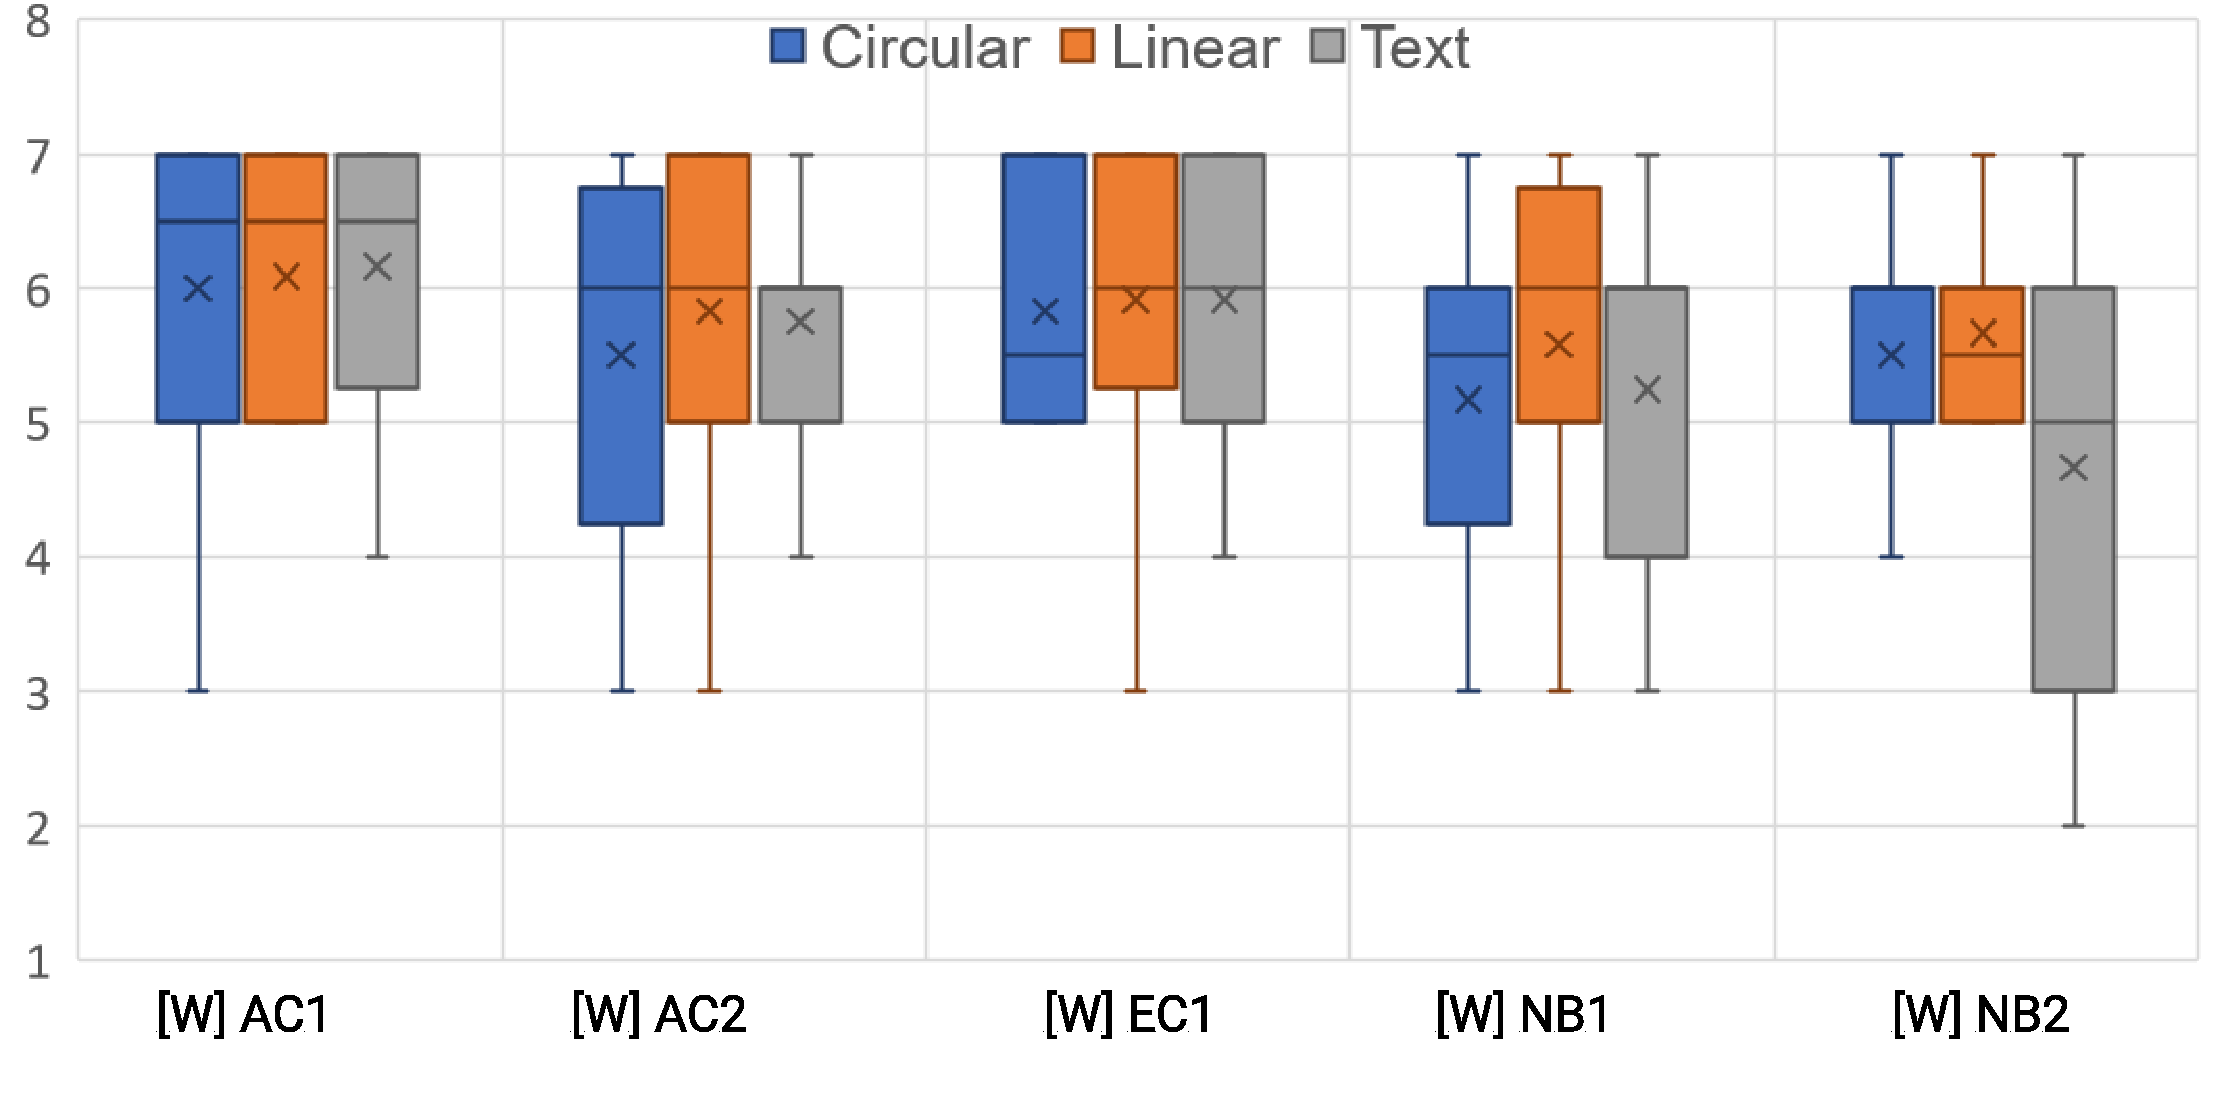
\includegraphics[width=\textwidth]{\Pic{study2/study2_box_receiver.pdf}}
  \caption{Perceived ratings by \receiver{} \prefixReceiver{}}
  \label{fig:Progressbar:study2:box_results_receiver}
\end{subfigure}
\begin{subfigure}{0.9\textwidth}
  \centering
  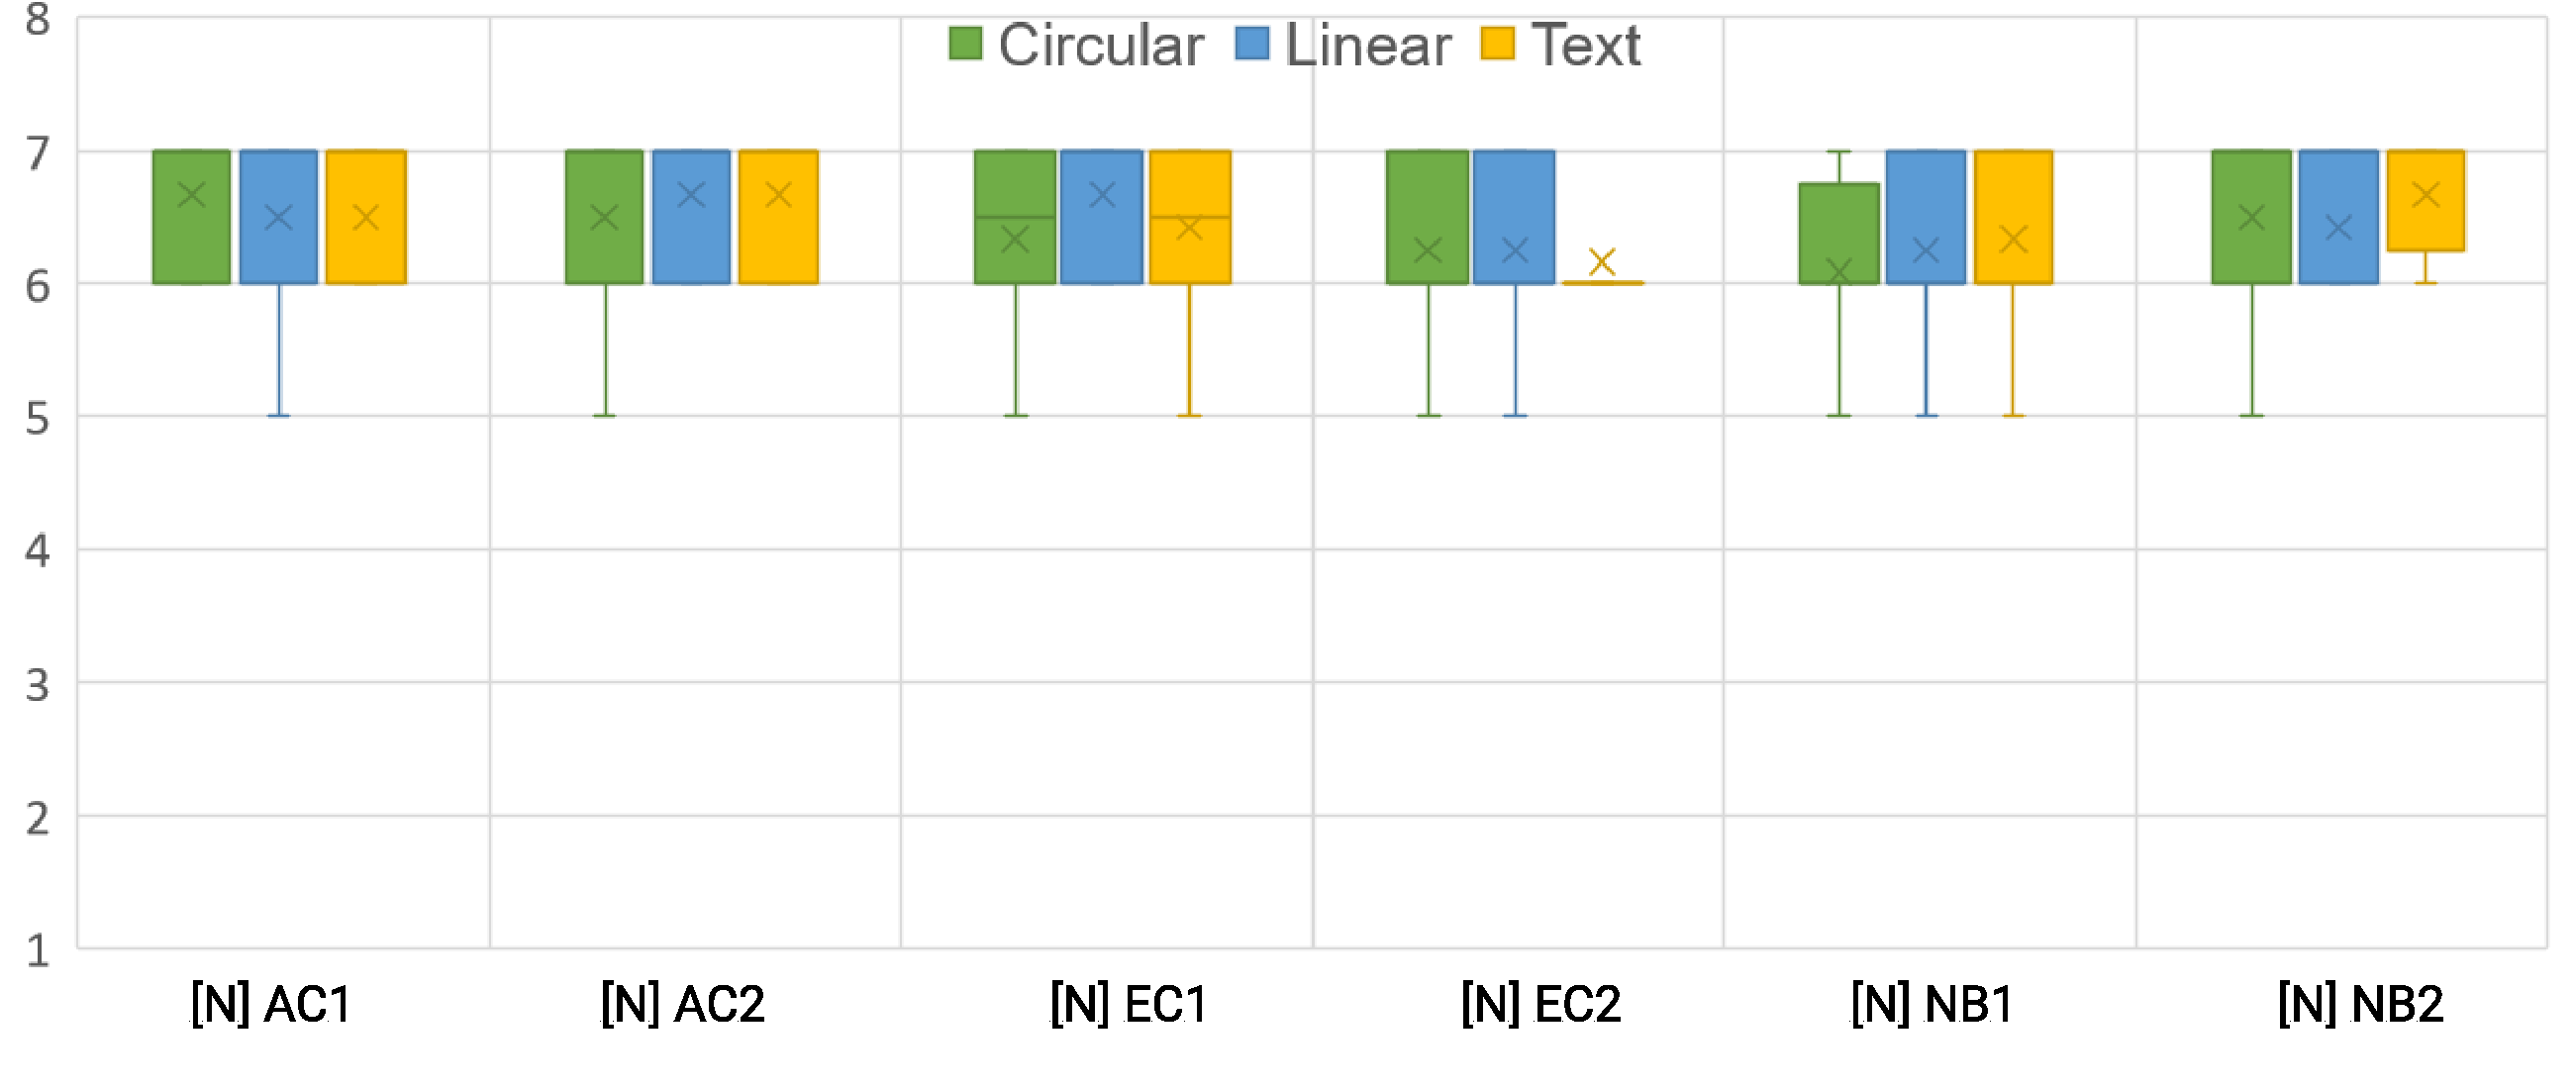
\includegraphics[width=\textwidth]{\Pic{study2/study2_box_observer.pdf}}
  \caption{Perceived ratings by \observer{} \prefixObserver{}}
  \label{fig:Progressbar:study2:box_results_observer}
\end{subfigure}

\caption[Primary task performance in \studytwo{}]{Perceived rating on progress \type{s} by \receiver{} \prefixReceiver{} and \observer{} \prefixObserver{} (N = 12).  $\times$ inside the box plot represents the mean value point. See  \autoref{tab:Progressbar:study2:measures_conversation} for details. }
\label{fig:Progressbar:study2:box_results}
\end{figure*}

\begin{table*}[hptb]
\centering
\caption[Average primary task performance in \studytwo{}]{Perceived rating in conversation setting (N = 12) by \receiver{} \prefixReceiver{} and \observer{} \prefixObserver{}. Here \i{C} = \Circularbar{}, \i{L} = \Linearbar{}, and \i{T} = \Textbar{}. Colored bars show the relative value of each measure for different progress \type{s}. \significantII{} and \significantIII{} represent non-significant (\pbonf{>0.05}) yet \pbonf{<0.10} post-hoc tests.}
\label{tab:Progressbar:study2:measures_conversation}

\scalebox{0.9}{
\begin{tabular}{@{}l|ll|ll|ll|ll|ll|ll@{}}
\toprule
\multicolumn{1}{r}{Measure} &
  \multicolumn{2}{c}{AC1} &
  \multicolumn{2}{c}{AC2} &
  \multicolumn{2}{c}{EC1} &
  \multicolumn{2}{c}{EC2}  &
  \multicolumn{2}{c}{NB1} & 
  \multicolumn{2}{c}{NB2} \\ \cmidrule(l){2-13} 
\multicolumn{1}{l}{Format} &
  \multicolumn{1}{l}{M} &
  \multicolumn{1}{l}{SD} &
  \multicolumn{1}{l}{M} &
  \multicolumn{1}{l}{SD} &
  \multicolumn{1}{l}{M} &
  \multicolumn{1}{l}{SD} &
  \multicolumn{1}{l}{M} &
  \multicolumn{1}{l}{SD} &
  \multicolumn{1}{l}{M} &
  \multicolumn{1}{l}{SD} &
  \multicolumn{1}{l}{M} &
  \multicolumn{1}{l}{SD} \\ \midrule
  
\prefixReceiver{} \i{C} & 
\databar{7}{6.00} & 1.28 & 
\databar{7}{5.50} & 1.31 &
\databar{7}{5.83} & 0.94 & 
- & - & 
\databar{7}{5.17} & 1.27 & 
\databar{7}{5.50}\significantII{} & 0.91 \\

\prefixReceiver{} \i{L} & 
\databar{7}{6.08} & 1.00 & 
\databar{7}{5.83} & 1.19 & 
\databar{7}{5.92} & 1.17 & 
- & - & 
\databar{7}{5.58} & 1.24 & 
\databar{7}{5.67}\significantIII{} & 0.78  \\

\prefixReceiver{} \i{T} & 
\databar{7}{6.17} & 1.03 & 
\databar{7}{5.75} & 0.87 & 
\databar{7}{5.92} & 1.17 & 
- & - & 
\databar{7}{5.25} & 1.22 &   
\databar{7}{4.67}\significantII{}\significantIII{} & 1.56  \\
\midrule

\prefixObserver{} \i{C} & 
\databar{7}{6.67} & 0.49 & 
\databar{7}{6.50} & 0.65 &
\databar{7}{6.33} & 0.78 & 
\databar{7}{6.25} & 0.75 & 
\databar{7}{6.08} & 0.67 & 
\databar{7}{6.50} & 0.67 \\

\prefixObserver{} \i{L} & 
\databar{7}{6.50} & 0.67 & 
\databar{7}{6.67} & 0.49 & 
\databar{7}{6.67} & 0.49 & 
\databar{7}{6.25} & 0.62 & 
\databar{7}{6.25} & 0.62 & 
\databar{7}{6.42} & 0.90  \\

\prefixObserver{} \i{T} & 
\databar{7}{6.50} & 0.91 & 
\databar{7}{6.67} & 0.49 & 
\databar{7}{6.42} & 0.67 & 
\databar{7}{6.17} & 0.39 &  
\databar{7}{6.33} & 0.65 &   
\databar{7}{6.67} & 0.65  \\

\bottomrule
\end{tabular}
}
\end{table*}


At the start, the \observer{s} felt \quote{uncomfortable} and \quote{awkward} talking with \receiver{s} who were wearing \quote{bulky} OHMDs but eventually found it more natural once the conversation began. They mentioned that using \quote{spectacle-like} OHMDs in a casual conversation would be socially acceptable, as it would be similar to the use of smartphones when engaged in a conversation, but still considered \quote{rude} in a professional setting. This could be because the Microsoft Hololens2 is still too bulky and does not resemble regular glasses. We expect this problem to be mitigated with more lightweight and natural-looking glasses such as the North Focals\footnote{\url{https://www.theverge.com/2019/2/14/18223593/focals-smart-glasses-north-review-specs-features-price}} smart glasses.

From the \observer{'s} point of view, they did not notice any significant differences in the naturalness of conversation among sessions. Sometimes, they noticed that the \receiver{s'} gaze \quote{moved to the corner}, but they assumed the \receiver{s} were thinking, and this was perceived as natural.


\subsubsection*{Progress perception (notification task performance).\\}

The post-hoc analysis showed that the \circularbar{} had the highest \noticeability{} and \perceivedEffectiveness{} compared with the \linearbar{} and \textbar{}, and a higher \comfortability{} compared with the \textbar{}. The Friedman test revealed significant differences between progress \type{s} in terms of \noticeability{} (\friedman{2}{8.600}{=0.014}{0.580}), \comfortability{} (\friedman{2}{6.324}{=0.042}{0.515}), and \perceivedEffectiveness{} (\friedman{2}{8.424}{=0.015}{0.696}). The differences between \circularbar{} and \linearbar{} in terms of \noticeability{} and \perceivedEffectiveness{} were significant (\pbonf{<0.05}), whereas the difference in terms of \comfortability{} was not significant (\pbonf{=0.098}). The detailed results are summarized in \autoref{fig:Progressbar:study2:box_progress_perception} (\autoref{tab:Progressbar:study2:measures_progress}).


\begin{figure}[hptb]
\centering
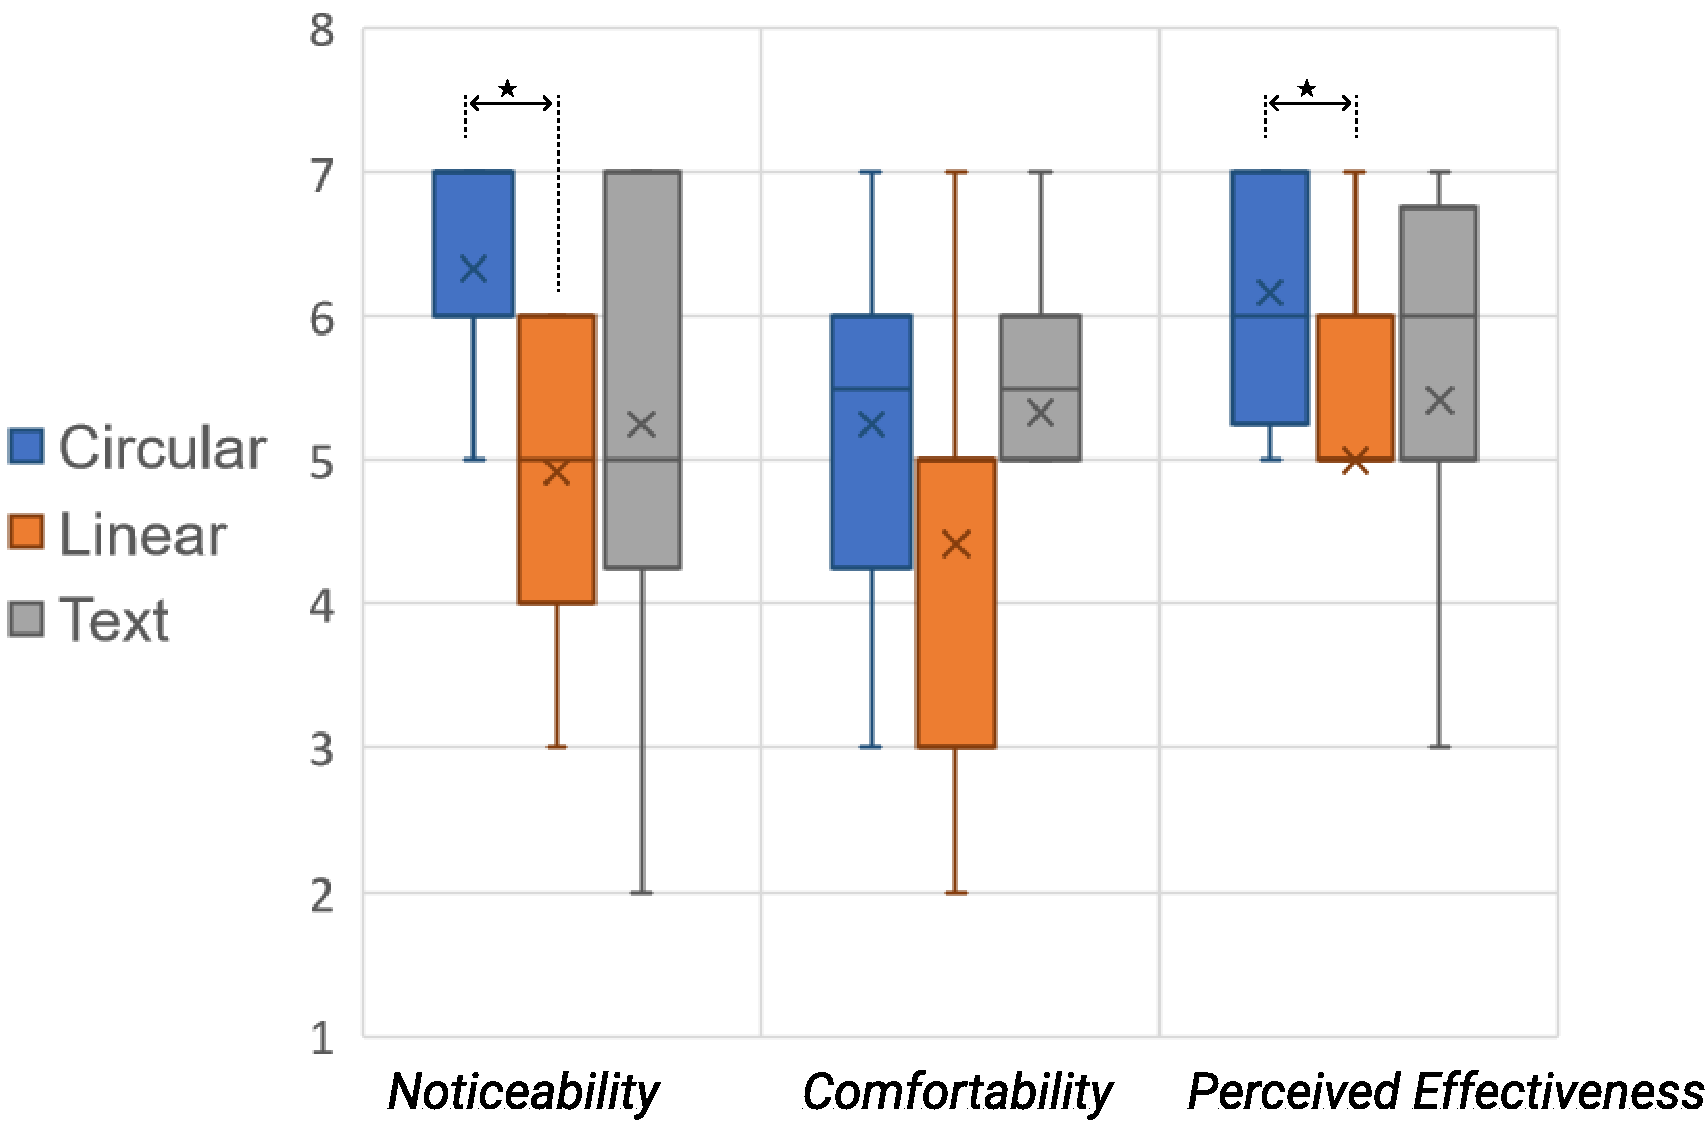
\includegraphics[width=0.65\linewidth]{\Pic{study2/study2_box_progress_perception.pdf}}
\caption[Secondary task performance in \studytwo{} by \receiver{}]{Perceived rating on progress \type{s} by \receiver{} (N = 12). \significantI{} represents significant (\pbonf{<0.05}) post-hoc tests and $\times$ inside box plot represents the mean value point. See \autoref{tab:Progressbar:study2:measures_progress} for details. }
\label{fig:Progressbar:study2:box_progress_perception}
\end{figure}


\begin{table*}[hptb]
\centering
\caption[Average secondary task performance in \studytwo{}]{Perceived rating on progress \type{s} (N = 12). Colored bars show the relative value of each measure for different progress \type{s}. \significantI{} represents significant (\pval{<0.05}) post-hoc tests. \significantII{} and \significantIII{} represents non-significant (\pbonf{>0.05}) yet \pbonf{<0.10} post-hoc tests.}
\label{tab:Progressbar:study2:measures_progress}
\small
\begin{tabular}{@{}l|ll|ll|ll@{}}
\toprule
\multicolumn{1}{r}{Measure} &
  \multicolumn{2}{c}{\noticeability{}} &
  \multicolumn{2}{c}{\comfortability{}}  &
  \multicolumn{2}{c}{\perceivedEffectiveness{}} \\ \cmidrule(l){2-7} 
\multicolumn{1}{l}{Format} &
  \multicolumn{1}{l}{M} &
  \multicolumn{1}{l}{SD} &
  \multicolumn{1}{l}{M} &
  \multicolumn{1}{l}{SD} &
  \multicolumn{1}{l}{M} &
  \multicolumn{1}{l}{SD} \\ \midrule
  
\Circularbar{} & 
\databar{7}{6.33}\significantI{} & 0.99 &
\databar{7}{5.25}\significantII{} & 1.14 & 
\databar{7}{6.17}\significantI{} & 0.84  \\

\Linearbar{} & 
\databar{7}{4.92}\significantI{} & 1.17 & 
\databar{7}{4.42}\significantII{}\significantIII{}  & 1.44 & 
\databar{7}{5.00}\significantI{} & 1.54 \\

\Textbar{} & 
\databar{7}{5.25} & 1.66 & 
\databar{7}{5.33}\significantIII{} & 1.30 & 
\databar{7}{5.42} & 1.56 \\

\bottomrule
\end{tabular}
\end{table*}


During the interview, all \receiver{s} mentioned that although they needed \quote{a short time} to glance at the progress bars, they did not have to look away from their partner for the \circularbar{} condition. However, for the \textbar{} and \linearbar{}, they needed to look at the top of the screen to check the progress.
While they could still maintain eye contact with the \observer{}, a few \receiver{s} (4/12) acknowledged that the sudden appearance of progress bars distracted them from their conversations. This distraction was relatively subtle, as the progress bars did not block their view of the \observer{} and only appeared intermittently. But they felt time pressure when the progress reached the end.


\subsubsection*{\Receiver{s'} preference}
\label{sec:Progressbar:study2:receiver_preference}

As shown in \autoref{fig:Progressbar:study2:overall_ranking}, more than half of the participants (7/12) ranked \circularbar{} as their highest preference, while 3 participants ranked \textbar{} and 2 participants ranked \linearbar{} as their most preferred.

\begin{figure}[hptb]
  \centering
  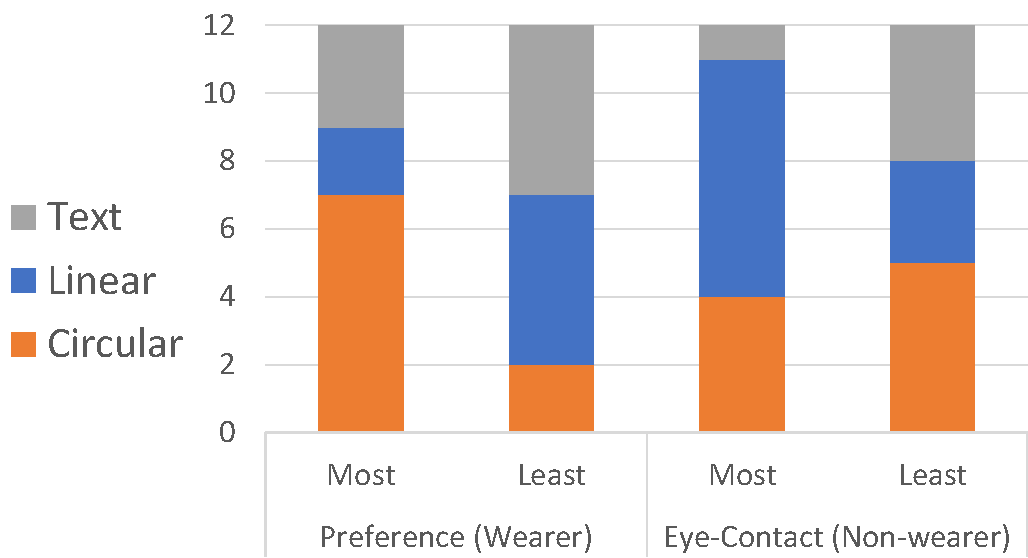
\includegraphics[width=0.65\linewidth]{\Pic{study2/study2_preference_distraction.pdf}}
  \caption[Overall preference in \studytwo{}]{Overall preference from \receiver{'s} perspective and eye contact ranking from \observer{'s} perspective}
  \label{fig:Progressbar:study2:overall_ranking}	  
\end{figure}




During the interview, participants who preferred \circularbar{} reported that it was easier to notice. The surrounding shape and the clock-like design enabled them to easily recognize the progress while maintaining attention on their partners. Compared with the \circularbar{}, the \linearbar{} required them to shift their attention away from the partner to see the progress. The \textbar{} was even harder to notice, required more attention to read the text, and was perceived as more \quote{stressful} as it provided exact numbers.

However, some participants did not prefer \circularbar{}, mentioning that the progress position of the \circularbar{} moved around the face, so they needed more time to check where to look. The \textbar{} and \linearbar{} were in a relatively fixed position, so they only needed to focus on one area to read progress.\\ 

\textit{\Observer{s'} perception of \receiver{s'} eye contact:}
Observers did not detect many differences in eye contact among the different conditions, although they did sometimes notice the participant looking up or to the side, but they interpreted this as \quote{they were processing what was said} or \quote{thinking about what to say next}, and did not take this as a lack of eye contact. As the \linearbar{} was placed above the head, when the \receiver{} looked at it, this could have been mistaken for thinking, but overall, this behavior did not cause any discomfort to \observer{s}.

\subsection{Discussion}

Overall, the majority (7/12) of \receiver{s} chose \circularbar{} as their first preference, which is consistent with \studyone{}, thus \circularbar{} is preferred over \linearbar{} and \textbar{}, is validated in a more realistic setting.
In accordance with \studyone{}, this study showed the \circularbar{} had higher noticeability and comfortability, and was also perceived as most effective in delivering progress information.

However, some participants (3/12) perceived the \textbar{} to be more comfortable for checking progress, as they could \quote{quickly glance} at the progress without significantly affecting social engagement. These three participants chose the \textbar{} as their first preference, indicating that it could also be suitable for certain users.

Except for the relaxation measure (i.e., \textit{NB2}), there were no significant differences between progress \type{s} on conversation quality. The \circularbar{} and \linearbar{} were \textit{more relaxing} to see than \textbar{} while conversing. Thus, statistically significant evidence is lacking to support that the \circularbar{} enables greater attention toward conversations. However, qualitative feedback supports the insight that \circularbar{} minimizes attention switching between conversation partner and on-screen progress information. Multiple participants mentioned how the information shown on the \circularbar{} is \quote{immediately understandable}, due to the shape and the graphical representation, meaning that they did not have to spend too much time processing the information and could continue conversing with their partner. They also mentioned how it was very \quote{obvious}, and could thus focus more on the primary task than interpreting or anticipating the progress bar.

Overall, based on the study results, we recommend using \circularbar{} to present progress/task completion notifications in face-to-face (1:1) conversations. But there are many other social interactions such as interviews, group meetings, and public speaking where progress notifications can be used, and we need further explorations to identify the most suitable \type{} in those scenarios and how they will be moderated by the urgency and importance of such notifications.























\section{General discussion}
\label{sec:Progressbar:general_discussion}

\subsection{Study summary}

In \studyone{}, we found that when participants maintained uninterrupted eye contact in a simulated conversational setting, the \circularbar{} enabled participants to receive progress notifications with less distraction, higher noticeability, comfortability, and accuracy. The \circularbar{}, aligned with the ring-shaped paracentral and near-peripheral vision, allowed users to interpret progress values with significantly higher accuracy than the \textbar{}. This was the preferred presentation type for the majority (83\%) of participants.
In \studytwo{}, we sought to verify the results of \studyone{} in a realistic conversation setting. We found that the \circularbar{} was perceived as more effective in notifying participants of progress. Participants felt more relaxed with the \circularbar{} than with the \textbar{}, and the majority of users (58\%) preferred it.
While the general consensus favored the \circularbar{}, there are merits to the other two designs.

As previously discussed, text is the most concise and direct presentation form but requires a certain amount of visual capability for viewing. The \linearbar{} strikes a balance between noticeability and disruption but provides an uneven viewing experience: the areas of the bar closer to the region of central vision are more visible than areas of the bar that are further away. The \circularbar{} and its circular shape make it easier to focus on the central location of the primary visual target, though its larger area can also be overwhelming. We analyzed these design trade-offs for deeper insights.

\begin{figure}[hptb]

\begin{subfigure}{1\linewidth}
  \centering
  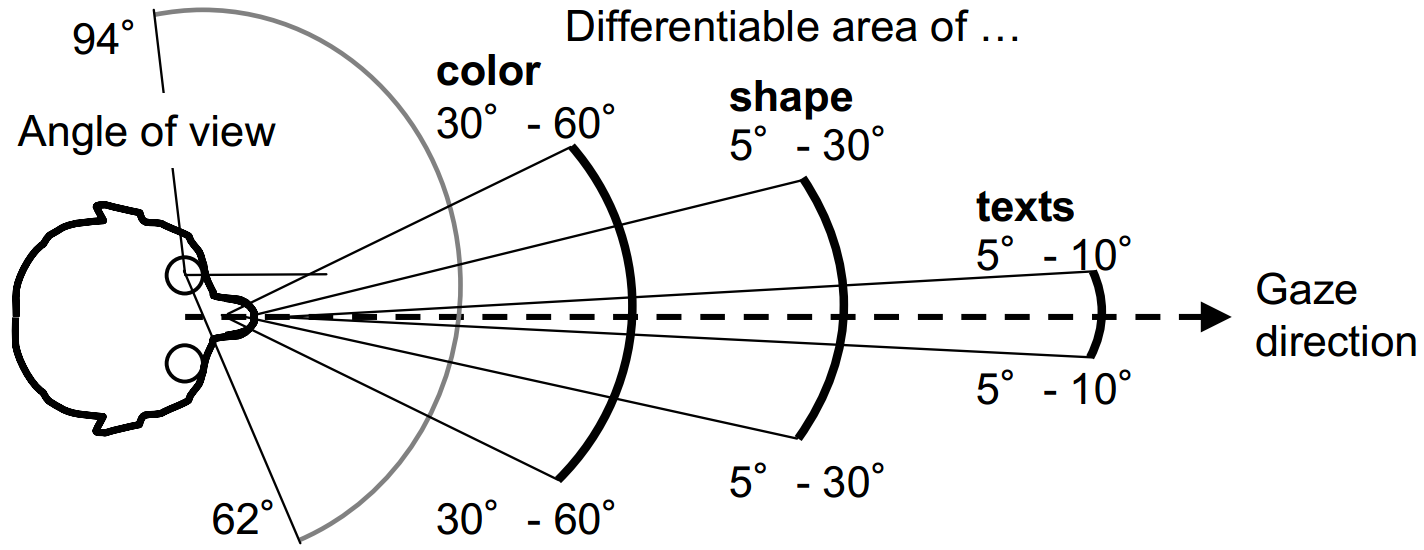
\includegraphics[width=0.72\linewidth]{\Pic{discussion/visual_perception_angles.png}}
  \caption{Visual perception angles of eyes. Source: \cite{ishiguro_peripheral_2011} (Figure~4).}
\end{subfigure}
\begin{subfigure}{1\linewidth}
  \centering
  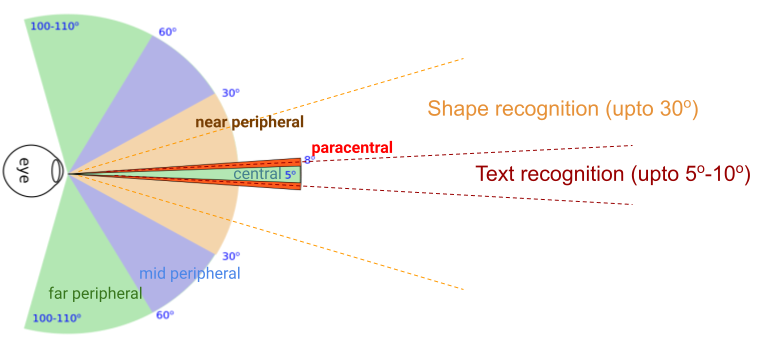
\includegraphics[width=0.9\linewidth]{\Pic{discussion/vision_capabilities.png}}
  \caption{Capabilities of paracentral and near-peripheral vision. References: \cite{wiki_fov_2021, ishiguro_peripheral_2011, panero1979human} }	  
\end{subfigure}

\caption[Visual perception angles of eyes]{Visual perception angles and capabilities of eyes for text, shapes, and color recognition.}
\label{fig:IconNotif:discussion:visual_perception}
\end{figure}

\subsection{The role of text in secondary information display}

As depicted in \autoref{fig:IconNotif:discussion:visual_perception}, even though the paracentral and near-peripheral regions possess some capability to recognize text or symbols, it remains challenging for most participants to reliably read text using either the paracentral or near-peripheral regions alone. Therefore, displaying text entirely outside the central vision is not recommended. However, our experiment also revealed that participants could largely discern the meaning of the text information in the paracentral vision, indicating a potential to offload some tasks from the central vision. One possible design is shown in \autoref{fig:Progressbar:discussion:circular_widgets}a. By placing the words across near-peripheral, paracentral, and central vision, the likelihood of comprehending the meaning significantly increases. While the text further away from the central vision is harder to read, readers can infer their meanings by considering them in conjunction with the text displayed in the central vision based on their context. We believe this strategy can be used to display familiar phrases while preserving the central vision for primary viewing tasks. Additionally, fonts designed specifically for peripheral viewing like `Eido' \cite{bernard_new_2016} or `PeriText' \cite{ku_peritext_2019}, can be employed for displaying text in the peripheral region of the eyes.

\begin{figure}[hptb]
  \centering
  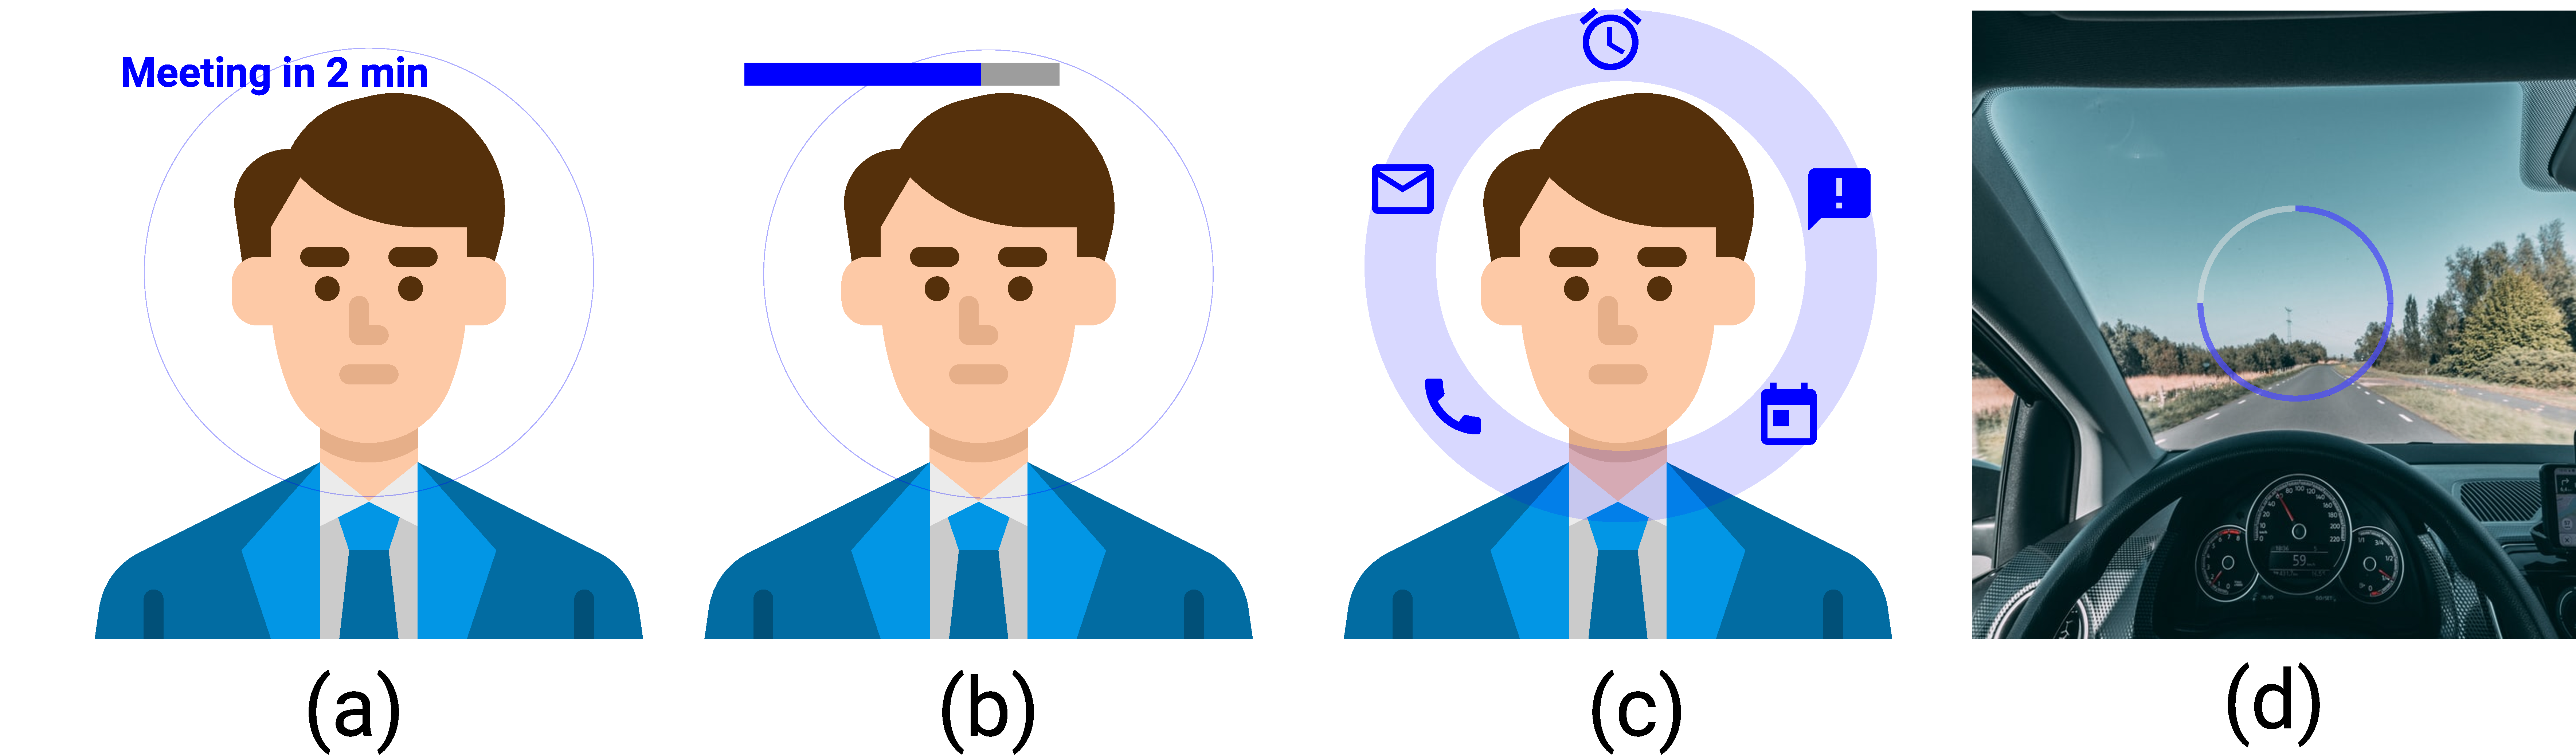
\includegraphics[width=0.9\linewidth]{\Pic{discussion/discussion_circular_widgets.pdf}}
  \caption[Applications scenarios of paracentral and near-peripheral visualization]{(a) Align important text to paracentral region, (b) Proposed \linearbar{}, (c) Use of paracentral and near-peripheral vision for a glanceable radial menu or notification display, (d) Use of paracentral vision to show  estimated arrival time. Image sources:  Flaticon.com (photo3idea\_studio), Unsplash.com, and Google Material Icons}
  \label{fig:Progressbar:discussion:circular_widgets}	  
\end{figure}



\subsection{Trade-off between circular vs. linear visualization}

We discovered that the circular shape offers a unique advantage as it mirrors the shape of our vision systems. By evenly distributing information around the central vision, it is easier for the user to maintain focus. Thus, a circle is an ideal shape for designing attention-maintaining secondary visual displays. This chapter explored one type of circular secondary information: progress updates, but this concept can be extended to other types of information. For instance, \autoref{fig:Progressbar:discussion:circular_widgets}c displays a transparent radial menu around the primary visual target. We believe such designs can help users perceive the menu options while easily maintaining visual focus. Another example is a modified notification summarizer, the `Scope', proposed by Dantzich et al. \cite{van_dantzich_scope_2002}, which leaves the center blank and puts notifications around the ring, allowing for multiple glanceable categories of notifications (\autoref{fig:Progressbar:discussion:circular_widgets}c). A similar design could also be used in presenting trip status (e.g., estimated arrival time) to users as shown in \autoref{fig:Progressbar:discussion:circular_widgets}d.

The \linearbar{}, although familiar, doesn't align well with our eyes' anatomy. However, the linear progress update visualization is more predictable as it consistently appears above the head (\autoref{sec:Progressbar:study2:receiver_preference}), thus easier for users to locate. Given that we understand the importance of progress information is not evenly distributed (more discussion in the following section): the closer to the deadline, the more critical the progress update becomes, so we could adjust the position of the \linearbar{} so that the ending segment is closer to the central vision (\autoref{fig:Progressbar:discussion:circular_widgets}b), thereby making it easier to perceive the information at the most important moments.

\subsection{Timing of progress update}

During the interview of \studytwo{}, we collected participants' feedback on the \intermittent{} \persistence{} of progress bars. Most participants (\receiver{s}) reported that they only checked the progress at the beginning and near the end of the conversation. Many of them (6/12) preferred the progress bar to appear \intermittent{ly} with a lower frequency (e.g., 25\%, 50\%, 75\%) at the beginning and to appear \intermittent{ly} with a higher frequency (e.g., 80\%, 90\%, 100\%) or even \continuous{ly} near the end. These results suggest that people's needs for checking the progress on the notification bar vary. They are particularly interested in being notified towards the end of the progress to prepare for follow-up actions. Thus, we recommend designing the \circularbar{} with a hybrid \persistence{}, supporting user customization.

\subsection{Social distance and perception of progress bars}

In realistic conversations, the distance between the \receiver{} and \observer{} can be shorter or longer than the distance we tested. When they get closer, the progress bars will move from the paracentral to near-peripheral to far-peripheral vision. In this situation, the \circularbar{} and the \linearbar{} can still be recognized due to their shape, but the \textbar{} would be harder to view unless they look up directly (assuming all progress bars maintain a fixed size). Similarly, if the distance between the \receiver{} and \observer{} increases, the progress bars will move from paracentral to central vision, where \receiver{s} may be able to derive precise information from the \textbar{} (if the font size remains visible). The \circularbar{} would still facilitate accurate estimation, while the \linearbar{} would be harder to estimate due to shortening of perception length. While our study provides a promising initial set of results, further research is needed to understand how the size and position of the secondary information interplay with the social distance between conversation partners.

\subsection{Attention-maintaining secondary information display design}

As we mentioned in the introduction, we increasingly encounter multitasking scenarios where multiple sources of information need to be attended to in a very short period or almost simultaneously. In such situations, it's essential to design visualizations that match the priority of the information source and the amount of attention it commands. A visualization that is unimportant but attention-grabbing is highly undesirable; a visual design that carefully considers the priority of its attention demand will be more visually pleasing. Our visual system has naturally evolved to have multiple regions responsible for different sources of information. These regions are equipped with different capabilities to naturally help us prioritize the information we receive. While previous research has explored the usage of central vision, mid and far peripheral vision subsystems, we believe the paracentral and near-peripheral vision is also worth investigating as they have different capabilities compared to other visual regions. This chapter conducted an initial investigation to demonstrate that these areas can be utilized to achieve better attention-maintaining secondary information displays. However, realizing their full potential requires further investigation. These include in-depth investigations comparing visual regions (e.g., central vs. paracentral), exploring their capabilities and capacities, determining optimal information distribution ratios, and more. We hope this chapter can increase awareness of this research topic, as we anticipate a possible paradigm shift towards heads-up and wearable computing. This line of research can aid future designers in developing better visualization techniques to mediate multiple information sources.










\section{Limitations}
\label{sec:Progressbar:limitations}

In \studyone{}, despite our usage of the gaze cursor and target regions, we were unable to control which vision region participants employed to check the progress values. Since we could not record the vision region (i.e., paracentral or near-peripheral) each individual used to inspect progress bars, we cannot conclusively state which region contributed more to the current results. This study represents an initial step towards understanding the use of paracentral and near-peripheral visualizations for OHMDs, and further studies are needed to precisely identify the advantages of each region.

While we strived to recreate a realistic scenario of casual conversations between participant pairs in \studytwo{}, the context and setting remained artificial. Conversation topics were predetermined and supplied to participants who were asked to maintain a fixed distance from each other. Although training was provided to minimize the effects of unfamiliarity, this factor may still have influenced participant engagement. Furthermore, as the studies progressed, \observer{s} might have grown more familiar with \studytwo{}, thereby affecting their ratings, even though they were blind to the conditions. While the speaker's turn may have influenced the perception of progress bars, the random nature of the turn-taking process indicates that it may not have favored any specific progress bar. Due to COVID-19 restrictions, all participants wore masks during the studies, potentially hindering non-verbal communication, with the exception of eye contact. However, the majority of participants (75\%) reported feeling that conversations felt natural once they began. We acknowledge the need for further studies to confirm whether these results are replicable in other realistic settings, such as during outdoor walking.











\section{Programming codes}
\label{sec:Progressbar:programming_codes}

\begin{sloppypar}
  The programming code for this chapter can be found at \url{https://github.com/NUS-HCILab/CircularProgressBar}.
\end{sloppypar}


\section{Conclusion}

We investigated the presentation of secondary information in paracentral and near-peripheral vision using OHMDs and demonstrated its potential to balance the reception of secondary information with the quality of social interaction. We introduced the \circularbar{}, a design that displays progress information in paracentral and near-peripheral vision during face-to-face conversations. By comparing the \circularbar{} with \linearbar{} and \textbar{} in both simulated and realistic conversational settings, we found that most users favored the \circularbar{}. It effectively conveys progress information to users without necessitating a break in eye contact with conversation partners. Future work could explore additional design solutions that leverage paracentral and near-peripheral vision in diverse multitasking scenarios.

These results offer an answer to our thesis question (\autoref{sec:Intro:thesis_RQ}): We can effectively decrease the attention costs associated with OHMD notifications during multitasking by utilizing different visual regions to distribute notification content based on its importance.

\subsubsection*{Summary of statistically significant results:}
{\small
\begin{itemize}
    \item In the simulated (lab) setting, 
    \begin{itemize}
        \item \Textbar{} led to higher perceived interruption than \linearbar{} and \circularbar{}.
        \item \Circularbar{} exhibited greater recognition accuracy than \linearbar{} and \textbar{}.
        \item \Textbar{} was perceived as less noticeable and less comfortable than \linearbar{} and \circularbar{}.
         \item A majority of participants (83\%) selected \circularbar{} as their first preference.
    \end{itemize}
    \item In the realistic setting, 
    \begin{itemize}
        \item \Circularbar{} demonstrated higher noticeability and perceived effectiveness compared to \linearbar{}.
        \item A majority of participants (58\%) selected \circularbar{} as their first preference.
    \end{itemize}
\end{itemize}
}





